% This file is part of GUFI, which is part of MarFS, which is released
% under the BSD license.
%
%
% Copyright (c) 2017, Los Alamos National Security (LANS), LLC
% All rights reserved.
%
% Redistribution and use in source and binary forms, with or without modification,
% are permitted provided that the following conditions are met:
%
% 1. Redistributions of source code must retain the above copyright notice, this
% list of conditions and the following disclaimer.
%
% 2. Redistributions in binary form must reproduce the above copyright notice,
% this list of conditions and the following disclaimer in the documentation and/or
% other materials provided with the distribution.
%
% 3. Neither the name of the copyright holder nor the names of its contributors
% may be used to endorse or promote products derived from this software without
% specific prior written permission.
%
% THIS SOFTWARE IS PROVIDED BY THE COPYRIGHT HOLDERS AND CONTRIBUTORS "AS IS" AND
% ANY EXPRESS OR IMPLIED WARRANTIES, INCLUDING, BUT NOT LIMITED TO, THE IMPLIED
% WARRANTIES OF MERCHANTABILITY AND FITNESS FOR A PARTICULAR PURPOSE ARE DISCLAIMED.
% IN NO EVENT SHALL THE COPYRIGHT HOLDER OR CONTRIBUTORS BE LIABLE FOR ANY DIRECT,
% INDIRECT, INCIDENTAL, SPECIAL, EXEMPLARY, OR CONSEQUENTIAL DAMAGES (INCLUDING,
% BUT NOT LIMITED TO, PROCUREMENT OF SUBSTITUTE GOODS OR SERVICES; LOSS OF USE,
% DATA, OR PROFITS; OR BUSINESS INTERRUPTION) HOWEVER CAUSED AND ON ANY THEORY OF
% LIABILITY, WHETHER IN CONTRACT, STRICT LIABILITY, OR TORT (INCLUDING NEGLIGENCE
% OR OTHERWISE) ARISING IN ANY WAY OUT OF THE USE OF THIS SOFTWARE, EVEN IF
% ADVISED OF THE POSSIBILITY OF SUCH DAMAGE.
%
%
% From Los Alamos National Security, LLC:
% LA-CC-15-039
%
% Copyright (c) 2017, Los Alamos National Security, LLC All rights reserved.
% Copyright 2017. Los Alamos National Security, LLC. This software was produced
% under U.S. Government contract DE-AC52-06NA25396 for Los Alamos National
% Laboratory (LANL), which is operated by Los Alamos National Security, LLC for
% the U.S. Department of Energy. The U.S. Government has rights to use,
% reproduce, and distribute this software.  NEITHER THE GOVERNMENT NOR LOS
% ALAMOS NATIONAL SECURITY, LLC MAKES ANY WARRANTY, EXPRESS OR IMPLIED, OR
% ASSUMES ANY LIABILITY FOR THE USE OF THIS SOFTWARE.  If software is
% modified to produce derivative works, such modified software should be
% clearly marked, so as not to confuse it with the version available from
% LANL.
%
% THIS SOFTWARE IS PROVIDED BY LOS ALAMOS NATIONAL SECURITY, LLC AND CONTRIBUTORS
% "AS IS" AND ANY EXPRESS OR IMPLIED WARRANTIES, INCLUDING, BUT NOT LIMITED TO,
% THE IMPLIED WARRANTIES OF MERCHANTABILITY AND FITNESS FOR A PARTICULAR PURPOSE
% ARE DISCLAIMED. IN NO EVENT SHALL LOS ALAMOS NATIONAL SECURITY, LLC OR
% CONTRIBUTORS BE LIABLE FOR ANY DIRECT, INDIRECT, INCIDENTAL, SPECIAL,
% EXEMPLARY, OR CONSEQUENTIAL DAMAGES (INCLUDING, BUT NOT LIMITED TO, PROCUREMENT
% OF SUBSTITUTE GOODS OR SERVICES; LOSS OF USE, DATA, OR PROFITS; OR BUSINESS
% INTERRUPTION) HOWEVER CAUSED AND ON ANY THEORY OF LIABILITY, WHETHER IN
% CONTRACT, STRICT LIABILITY, OR TORT (INCLUDING NEGLIGENCE OR OTHERWISE) ARISING
% IN ANY WAY OUT OF THE USE OF THIS SOFTWARE, EVEN IF ADVISED OF THE POSSIBILITY
% OF SUCH DAMAGE.



\documentclass{article}

% Useful packages
\usepackage{graphicx}
\usepackage{hyperref}
\usepackage{rotating}
\usepackage{verbatim}
\usepackage{GUFIText}

\hypersetup{
    colorlinks,
    citecolor=black,
    filecolor=black,
    linkcolor=black,
    urlcolor=blue
}

\title{GUFI Administrator's Guide}
\author{GUFI Developers}

\begin{document}

\maketitle

\tableofcontents
% This file is part of GUFI, which is part of MarFS, which is released
% under the BSD license.
%
%
% Copyright (c) 2017, Los Alamos National Security (LANS), LLC
% All rights reserved.
%
% Redistribution and use in source and binary forms, with or without modification,
% are permitted provided that the following conditions are met:
%
% 1. Redistributions of source code must retain the above copyright notice, this
% list of conditions and the following disclaimer.
%
% 2. Redistributions in binary form must reproduce the above copyright notice,
% this list of conditions and the following disclaimer in the documentation and/or
% other materials provided with the distribution.
%
% 3. Neither the name of the copyright holder nor the names of its contributors
% may be used to endorse or promote products derived from this software without
% specific prior written permission.
%
% THIS SOFTWARE IS PROVIDED BY THE COPYRIGHT HOLDERS AND CONTRIBUTORS "AS IS" AND
% ANY EXPRESS OR IMPLIED WARRANTIES, INCLUDING, BUT NOT LIMITED TO, THE IMPLIED
% WARRANTIES OF MERCHANTABILITY AND FITNESS FOR A PARTICULAR PURPOSE ARE DISCLAIMED.
% IN NO EVENT SHALL THE COPYRIGHT HOLDER OR CONTRIBUTORS BE LIABLE FOR ANY DIRECT,
% INDIRECT, INCIDENTAL, SPECIAL, EXEMPLARY, OR CONSEQUENTIAL DAMAGES (INCLUDING,
% BUT NOT LIMITED TO, PROCUREMENT OF SUBSTITUTE GOODS OR SERVICES; LOSS OF USE,
% DATA, OR PROFITS; OR BUSINESS INTERRUPTION) HOWEVER CAUSED AND ON ANY THEORY OF
% LIABILITY, WHETHER IN CONTRACT, STRICT LIABILITY, OR TORT (INCLUDING NEGLIGENCE
% OR OTHERWISE) ARISING IN ANY WAY OUT OF THE USE OF THIS SOFTWARE, EVEN IF
% ADVISED OF THE POSSIBILITY OF SUCH DAMAGE.
%
%
% From Los Alamos National Security, LLC:
% LA-CC-15-039
%
% Copyright (c) 2017, Los Alamos National Security, LLC All rights reserved.
% Copyright 2017. Los Alamos National Security, LLC. This software was produced
% under U.S. Government contract DE-AC52-06NA25396 for Los Alamos National
% Laboratory (LANL), which is operated by Los Alamos National Security, LLC for
% the U.S. Department of Energy. The U.S. Government has rights to use,
% reproduce, and distribute this software.  NEITHER THE GOVERNMENT NOR LOS
% ALAMOS NATIONAL SECURITY, LLC MAKES ANY WARRANTY, EXPRESS OR IMPLIED, OR
% ASSUMES ANY LIABILITY FOR THE USE OF THIS SOFTWARE.  If software is
% modified to produce derivative works, such modified software should be
% clearly marked, so as not to confuse it with the version available from
% LANL.
%
% THIS SOFTWARE IS PROVIDED BY LOS ALAMOS NATIONAL SECURITY, LLC AND CONTRIBUTORS
% "AS IS" AND ANY EXPRESS OR IMPLIED WARRANTIES, INCLUDING, BUT NOT LIMITED TO,
% THE IMPLIED WARRANTIES OF MERCHANTABILITY AND FITNESS FOR A PARTICULAR PURPOSE
% ARE DISCLAIMED. IN NO EVENT SHALL LOS ALAMOS NATIONAL SECURITY, LLC OR
% CONTRIBUTORS BE LIABLE FOR ANY DIRECT, INDIRECT, INCIDENTAL, SPECIAL,
% EXEMPLARY, OR CONSEQUENTIAL DAMAGES (INCLUDING, BUT NOT LIMITED TO, PROCUREMENT
% OF SUBSTITUTE GOODS OR SERVICES; LOSS OF USE, DATA, OR PROFITS; OR BUSINESS
% INTERRUPTION) HOWEVER CAUSED AND ON ANY THEORY OF LIABILITY, WHETHER IN
% CONTRACT, STRICT LIABILITY, OR TORT (INCLUDING NEGLIGENCE OR OTHERWISE) ARISING
% IN ANY WAY OUT OF THE USE OF THIS SOFTWARE, EVEN IF ADVISED OF THE POSSIBILITY
% OF SUCH DAMAGE.



\section{License}
\verbatiminput{../../../../LICENSE.txt}

% This file is part of GUFI, which is part of MarFS, which is released
% under the BSD license.
%
%
% Copyright (c) 2017, Los Alamos National Security (LANS), LLC
% All rights reserved.
%
% Redistribution and use in source and binary forms, with or without modification,
% are permitted provided that the following conditions are met:
%
% 1. Redistributions of source code must retain the above copyright notice, this
% list of conditions and the following disclaimer.
%
% 2. Redistributions in binary form must reproduce the above copyright notice,
% this list of conditions and the following disclaimer in the documentation and/or
% other materials provided with the distribution.
%
% 3. Neither the name of the copyright holder nor the names of its contributors
% may be used to endorse or promote products derived from this software without
% specific prior written permission.
%
% THIS SOFTWARE IS PROVIDED BY THE COPYRIGHT HOLDERS AND CONTRIBUTORS "AS IS" AND
% ANY EXPRESS OR IMPLIED WARRANTIES, INCLUDING, BUT NOT LIMITED TO, THE IMPLIED
% WARRANTIES OF MERCHANTABILITY AND FITNESS FOR A PARTICULAR PURPOSE ARE DISCLAIMED.
% IN NO EVENT SHALL THE COPYRIGHT HOLDER OR CONTRIBUTORS BE LIABLE FOR ANY DIRECT,
% INDIRECT, INCIDENTAL, SPECIAL, EXEMPLARY, OR CONSEQUENTIAL DAMAGES (INCLUDING,
% BUT NOT LIMITED TO, PROCUREMENT OF SUBSTITUTE GOODS OR SERVICES; LOSS OF USE,
% DATA, OR PROFITS; OR BUSINESS INTERRUPTION) HOWEVER CAUSED AND ON ANY THEORY OF
% LIABILITY, WHETHER IN CONTRACT, STRICT LIABILITY, OR TORT (INCLUDING NEGLIGENCE
% OR OTHERWISE) ARISING IN ANY WAY OUT OF THE USE OF THIS SOFTWARE, EVEN IF
% ADVISED OF THE POSSIBILITY OF SUCH DAMAGE.
%
%
% From Los Alamos National Security, LLC:
% LA-CC-15-039
%
% Copyright (c) 2017, Los Alamos National Security, LLC All rights reserved.
% Copyright 2017. Los Alamos National Security, LLC. This software was produced
% under U.S. Government contract DE-AC52-06NA25396 for Los Alamos National
% Laboratory (LANL), which is operated by Los Alamos National Security, LLC for
% the U.S. Department of Energy. The U.S. Government has rights to use,
% reproduce, and distribute this software.  NEITHER THE GOVERNMENT NOR LOS
% ALAMOS NATIONAL SECURITY, LLC MAKES ANY WARRANTY, EXPRESS OR IMPLIED, OR
% ASSUMES ANY LIABILITY FOR THE USE OF THIS SOFTWARE.  If software is
% modified to produce derivative works, such modified software should be
% clearly marked, so as not to confuse it with the version available from
% LANL.
%
% THIS SOFTWARE IS PROVIDED BY LOS ALAMOS NATIONAL SECURITY, LLC AND CONTRIBUTORS
% "AS IS" AND ANY EXPRESS OR IMPLIED WARRANTIES, INCLUDING, BUT NOT LIMITED TO,
% THE IMPLIED WARRANTIES OF MERCHANTABILITY AND FITNESS FOR A PARTICULAR PURPOSE
% ARE DISCLAIMED. IN NO EVENT SHALL LOS ALAMOS NATIONAL SECURITY, LLC OR
% CONTRIBUTORS BE LIABLE FOR ANY DIRECT, INDIRECT, INCIDENTAL, SPECIAL,
% EXEMPLARY, OR CONSEQUENTIAL DAMAGES (INCLUDING, BUT NOT LIMITED TO, PROCUREMENT
% OF SUBSTITUTE GOODS OR SERVICES; LOSS OF USE, DATA, OR PROFITS; OR BUSINESS
% INTERRUPTION) HOWEVER CAUSED AND ON ANY THEORY OF LIABILITY, WHETHER IN
% CONTRACT, STRICT LIABILITY, OR TORT (INCLUDING NEGLIGENCE OR OTHERWISE) ARISING
% IN ANY WAY OUT OF THE USE OF THIS SOFTWARE, EVEN IF ADVISED OF THE POSSIBILITY
% OF SUCH DAMAGE.
\section{Introduction}
Over the years, the amount of data we store and use has grown exponentially to the point that petabytes of storage is not uncommon. What used to be a simple task of accessing and sorting through information has been compounded into an arduous task with the size and scale of super-computing data centers. Being able to query data effectively, while also taking into account permissions becomes paramount into accomplishing daily tasks. This is what the Grand Unified File Index(GUFI) tool aims to accomplish. 
\\
\\
This process of efficiently accessing data is accomplished by recreating the tree structure via indexing. Each directory contains an SQL database file that stores the metadata of the files as well as summary information for that directory and optionally summary information for the entire tree below that directory. 

\begin{figure} [h]
\centering
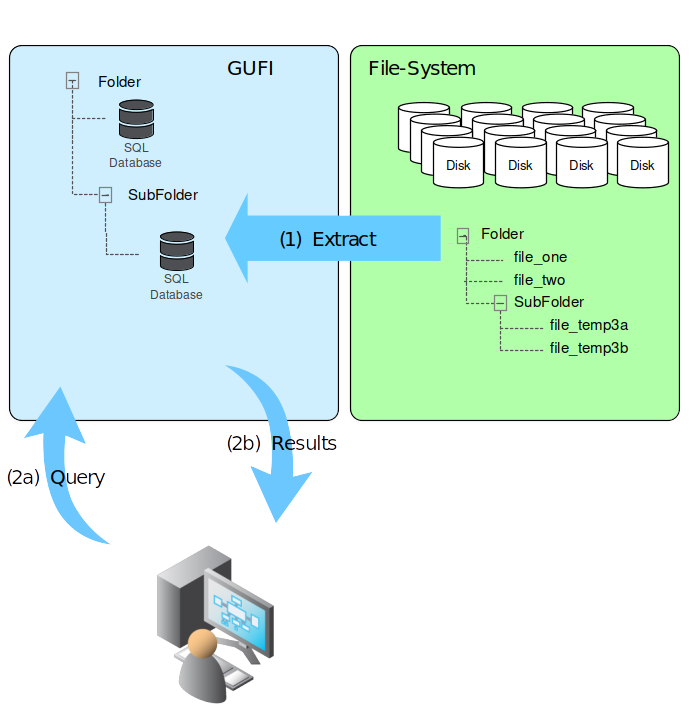
\includegraphics[width=0.5\textwidth]{images/gufi_structure.png}
\caption{\label{fig:gufi_structure}Layout and user interaction with GUFI}
\end{figure}

% This file is part of GUFI, which is part of MarFS, which is released
% under the BSD license.
%
%
% Copyright (c) 2017, Los Alamos National Security (LANS), LLC
% All rights reserved.
%
% Redistribution and use in source and binary forms, with or without modification,
% are permitted provided that the following conditions are met:
%
% 1. Redistributions of source code must retain the above copyright notice, this
% list of conditions and the following disclaimer.
%
% 2. Redistributions in binary form must reproduce the above copyright notice,
% this list of conditions and the following disclaimer in the documentation and/or
% other materials provided with the distribution.
%
% 3. Neither the name of the copyright holder nor the names of its contributors
% may be used to endorse or promote products derived from this software without
% specific prior written permission.
%
% THIS SOFTWARE IS PROVIDED BY THE COPYRIGHT HOLDERS AND CONTRIBUTORS "AS IS" AND
% ANY EXPRESS OR IMPLIED WARRANTIES, INCLUDING, BUT NOT LIMITED TO, THE IMPLIED
% WARRANTIES OF MERCHANTABILITY AND FITNESS FOR A PARTICULAR PURPOSE ARE DISCLAIMED.
% IN NO EVENT SHALL THE COPYRIGHT HOLDER OR CONTRIBUTORS BE LIABLE FOR ANY DIRECT,
% INDIRECT, INCIDENTAL, SPECIAL, EXEMPLARY, OR CONSEQUENTIAL DAMAGES (INCLUDING,
% BUT NOT LIMITED TO, PROCUREMENT OF SUBSTITUTE GOODS OR SERVICES; LOSS OF USE,
% DATA, OR PROFITS; OR BUSINESS INTERRUPTION) HOWEVER CAUSED AND ON ANY THEORY OF
% LIABILITY, WHETHER IN CONTRACT, STRICT LIABILITY, OR TORT (INCLUDING NEGLIGENCE
% OR OTHERWISE) ARISING IN ANY WAY OUT OF THE USE OF THIS SOFTWARE, EVEN IF
% ADVISED OF THE POSSIBILITY OF SUCH DAMAGE.
%
%
% From Los Alamos National Security, LLC:
% LA-CC-15-039
%
% Copyright (c) 2017, Los Alamos National Security, LLC All rights reserved.
% Copyright 2017. Los Alamos National Security, LLC. This software was produced
% under U.S. Government contract DE-AC52-06NA25396 for Los Alamos National
% Laboratory (LANL), which is operated by Los Alamos National Security, LLC for
% the U.S. Department of Energy. The U.S. Government has rights to use,
% reproduce, and distribute this software.  NEITHER THE GOVERNMENT NOR LOS
% ALAMOS NATIONAL SECURITY, LLC MAKES ANY WARRANTY, EXPRESS OR IMPLIED, OR
% ASSUMES ANY LIABILITY FOR THE USE OF THIS SOFTWARE.  If software is
% modified to produce derivative works, such modified software should be
% clearly marked, so as not to confuse it with the version available from
% LANL.
%
% THIS SOFTWARE IS PROVIDED BY LOS ALAMOS NATIONAL SECURITY, LLC AND CONTRIBUTORS
% "AS IS" AND ANY EXPRESS OR IMPLIED WARRANTIES, INCLUDING, BUT NOT LIMITED TO,
% THE IMPLIED WARRANTIES OF MERCHANTABILITY AND FITNESS FOR A PARTICULAR PURPOSE
% ARE DISCLAIMED. IN NO EVENT SHALL LOS ALAMOS NATIONAL SECURITY, LLC OR
% CONTRIBUTORS BE LIABLE FOR ANY DIRECT, INDIRECT, INCIDENTAL, SPECIAL,
% EXEMPLARY, OR CONSEQUENTIAL DAMAGES (INCLUDING, BUT NOT LIMITED TO, PROCUREMENT
% OF SUBSTITUTE GOODS OR SERVICES; LOSS OF USE, DATA, OR PROFITS; OR BUSINESS
% INTERRUPTION) HOWEVER CAUSED AND ON ANY THEORY OF LIABILITY, WHETHER IN
% CONTRACT, STRICT LIABILITY, OR TORT (INCLUDING NEGLIGENCE OR OTHERWISE) ARISING
% IN ANY WAY OUT OF THE USE OF THIS SOFTWARE, EVEN IF ADVISED OF THE POSSIBILITY
% OF SUCH DAMAGE.



\section{Dependencies}
A number of dependencies that should be installed before attempting to
build GUFI. There are also many optional dependencies that can enable
optional features.

\subsection{System Tools}
\begin{tabularx}{\textwidth}{| l | c | X | }
  \hline
  Package/Executable & Required? & Comments \\
  \hline
  autotools & Yes & Some bundled packages use autotools \\
  \hline
  C Compiler & Yes & C99 support \\
  \hline
  C++ Compiler & No & C++11 support - g++ 4.9.3, clang++-3.9, or newer
  \hfill \\
  \hline
  CMake & Yes & Version 3.1 or better \\
  \hline
  Make & Yes & \\
  \hline
  Python & Yes & Python 2.7 or Python 3 \\
  \hline
  pip & No & Used for installing and client dependencies \\
  \hline
  git & No & 1.8.5 or better if using the performance history
  framework \\
  \hline
  \LaTeX & No & Only needed if building \LaTeX \hfill \\
  & & Documentation \hfill \\
  \hline
  pkg-config & Yes & \\
  \hline
  realpath & Yes & \\
  \hline
  rpmbuild & No & Only needed if building RPMs \\
  \hline
  setfattr & Yes & attr package \\
  & & \texttt{xattr -w} on OSX \\
  \hline
  truncate & Yes & The -s option must be available \\
  \hline
  uname & No & Only needed if building RPMs \\
  \hline
\end{tabularx}

\subsection{Libraries}
\begin{tabularx}{\textwidth}{| l | c | X |}
  \hline
  Name & Required? & Comments \\
  \hline
  xattr & Yes & \\
  \hline
  pcre & Yes & Version 1 \\
  \hline
  mysql & No & \\
  \hline
  fuse & No & Called osxfuse on OSX \\
  \hline
  db2 & No & \\
  \hline
  gpfs & No & \\
  \hline
  matplotlib & No & Python library used for plotting numbers collected
  by the performance history framework \\
  \hline
\end{tabularx}

\subsection{Packages provided by GUFI}
Several packages are provided/downloaded, built, and installed
automatically:
\begin{tabularx}{\textwidth}{| l | X |}
  \hline
  Name & Comments \\
  \hline
  GoogleTest & \url{https://github.com/google/googletest} \\
  \hline
  jemalloc & \url{https://github.com/jemalloc/jemalloc} \\
  \hline
  paramiko & \url{https://github.com/paramiko/paramiko} \\
  & patched ae3d0febef17a8ece5268bbf6c210a30573ce800 \\
  & Use pip to download python-bcrypt, python-cryptography, and
  python-pynacl \\
  \hline
  sqlite3 & \url{https://www.sqlite.org/index.html} \\
  & patched sqlite-autoconf-3270200.tar.gz \\
  \hline
  sqlite3-pcre & \url{https://github.com/mar-file-system/sqlite3-pcre}
  \\
  \hline
\end{tabularx}

% This file is part of GUFI, which is part of MarFS, which is released
% under the BSD license.
%
%
% Copyright (c) 2017, Los Alamos National Security (LANS), LLC
% All rights reserved.
%
% Redistribution and use in source and binary forms, with or without modification,
% are permitted provided that the following conditions are met:
%
% 1. Redistributions of source code must retain the above copyright notice, this
% list of conditions and the following disclaimer.
%
% 2. Redistributions in binary form must reproduce the above copyright notice,
% this list of conditions and the following disclaimer in the documentation and/or
% other materials provided with the distribution.
%
% 3. Neither the name of the copyright holder nor the names of its contributors
% may be used to endorse or promote products derived from this software without
% specific prior written permission.
%
% THIS SOFTWARE IS PROVIDED BY THE COPYRIGHT HOLDERS AND CONTRIBUTORS "AS IS" AND
% ANY EXPRESS OR IMPLIED WARRANTIES, INCLUDING, BUT NOT LIMITED TO, THE IMPLIED
% WARRANTIES OF MERCHANTABILITY AND FITNESS FOR A PARTICULAR PURPOSE ARE DISCLAIMED.
% IN NO EVENT SHALL THE COPYRIGHT HOLDER OR CONTRIBUTORS BE LIABLE FOR ANY DIRECT,
% INDIRECT, INCIDENTAL, SPECIAL, EXEMPLARY, OR CONSEQUENTIAL DAMAGES (INCLUDING,
% BUT NOT LIMITED TO, PROCUREMENT OF SUBSTITUTE GOODS OR SERVICES; LOSS OF USE,
% DATA, OR PROFITS; OR BUSINESS INTERRUPTION) HOWEVER CAUSED AND ON ANY THEORY OF
% LIABILITY, WHETHER IN CONTRACT, STRICT LIABILITY, OR TORT (INCLUDING NEGLIGENCE
% OR OTHERWISE) ARISING IN ANY WAY OUT OF THE USE OF THIS SOFTWARE, EVEN IF
% ADVISED OF THE POSSIBILITY OF SUCH DAMAGE.
%
%
% From Los Alamos National Security, LLC:
% LA-CC-15-039
%
% Copyright (c) 2017, Los Alamos National Security, LLC All rights reserved.
% Copyright 2017. Los Alamos National Security, LLC. This software was produced
% under U.S. Government contract DE-AC52-06NA25396 for Los Alamos National
% Laboratory (LANL), which is operated by Los Alamos National Security, LLC for
% the U.S. Department of Energy. The U.S. Government has rights to use,
% reproduce, and distribute this software.  NEITHER THE GOVERNMENT NOR LOS
% ALAMOS NATIONAL SECURITY, LLC MAKES ANY WARRANTY, EXPRESS OR IMPLIED, OR
% ASSUMES ANY LIABILITY FOR THE USE OF THIS SOFTWARE.  If software is
% modified to produce derivative works, such modified software should be
% clearly marked, so as not to confuse it with the version available from
% LANL.
%
% THIS SOFTWARE IS PROVIDED BY LOS ALAMOS NATIONAL SECURITY, LLC AND CONTRIBUTORS
% "AS IS" AND ANY EXPRESS OR IMPLIED WARRANTIES, INCLUDING, BUT NOT LIMITED TO,
% THE IMPLIED WARRANTIES OF MERCHANTABILITY AND FITNESS FOR A PARTICULAR PURPOSE
% ARE DISCLAIMED. IN NO EVENT SHALL LOS ALAMOS NATIONAL SECURITY, LLC OR
% CONTRIBUTORS BE LIABLE FOR ANY DIRECT, INDIRECT, INCIDENTAL, SPECIAL,
% EXEMPLARY, OR CONSEQUENTIAL DAMAGES (INCLUDING, BUT NOT LIMITED TO, PROCUREMENT
% OF SUBSTITUTE GOODS OR SERVICES; LOSS OF USE, DATA, OR PROFITS; OR BUSINESS
% INTERRUPTION) HOWEVER CAUSED AND ON ANY THEORY OF LIABILITY, WHETHER IN
% CONTRACT, STRICT LIABILITY, OR TORT (INCLUDING NEGLIGENCE OR OTHERWISE) ARISING
% IN ANY WAY OUT OF THE USE OF THIS SOFTWARE, EVEN IF ADVISED OF THE POSSIBILITY
% OF SUCH DAMAGE.



\section{Download}

The source code for GUFI can be found at
\url{https://github.com/mar-file-system/GUFI}.

% This file is part of GUFI, which is part of MarFS, which is released
% under the BSD license.
%
%
% Copyright (c) 2017, Los Alamos National Security (LANS), LLC
% All rights reserved.
%
% Redistribution and use in source and binary forms, with or without modification,
% are permitted provided that the following conditions are met:
%
% 1. Redistributions of source code must retain the above copyright notice, this
% list of conditions and the following disclaimer.
%
% 2. Redistributions in binary form must reproduce the above copyright notice,
% this list of conditions and the following disclaimer in the documentation and/or
% other materials provided with the distribution.
%
% 3. Neither the name of the copyright holder nor the names of its contributors
% may be used to endorse or promote products derived from this software without
% specific prior written permission.
%
% THIS SOFTWARE IS PROVIDED BY THE COPYRIGHT HOLDERS AND CONTRIBUTORS "AS IS" AND
% ANY EXPRESS OR IMPLIED WARRANTIES, INCLUDING, BUT NOT LIMITED TO, THE IMPLIED
% WARRANTIES OF MERCHANTABILITY AND FITNESS FOR A PARTICULAR PURPOSE ARE DISCLAIMED.
% IN NO EVENT SHALL THE COPYRIGHT HOLDER OR CONTRIBUTORS BE LIABLE FOR ANY DIRECT,
% INDIRECT, INCIDENTAL, SPECIAL, EXEMPLARY, OR CONSEQUENTIAL DAMAGES (INCLUDING,
% BUT NOT LIMITED TO, PROCUREMENT OF SUBSTITUTE GOODS OR SERVICES; LOSS OF USE,
% DATA, OR PROFITS; OR BUSINESS INTERRUPTION) HOWEVER CAUSED AND ON ANY THEORY OF
% LIABILITY, WHETHER IN CONTRACT, STRICT LIABILITY, OR TORT (INCLUDING NEGLIGENCE
% OR OTHERWISE) ARISING IN ANY WAY OUT OF THE USE OF THIS SOFTWARE, EVEN IF
% ADVISED OF THE POSSIBILITY OF SUCH DAMAGE.
%
%
% From Los Alamos National Security, LLC:
% LA-CC-15-039
%
% Copyright (c) 2017, Los Alamos National Security, LLC All rights reserved.
% Copyright 2017. Los Alamos National Security, LLC. This software was produced
% under U.S. Government contract DE-AC52-06NA25396 for Los Alamos National
% Laboratory (LANL), which is operated by Los Alamos National Security, LLC for
% the U.S. Department of Energy. The U.S. Government has rights to use,
% reproduce, and distribute this software.  NEITHER THE GOVERNMENT NOR LOS
% ALAMOS NATIONAL SECURITY, LLC MAKES ANY WARRANTY, EXPRESS OR IMPLIED, OR
% ASSUMES ANY LIABILITY FOR THE USE OF THIS SOFTWARE.  If software is
% modified to produce derivative works, such modified software should be
% clearly marked, so as not to confuse it with the version available from
% LANL.
%
% THIS SOFTWARE IS PROVIDED BY LOS ALAMOS NATIONAL SECURITY, LLC AND CONTRIBUTORS
% "AS IS" AND ANY EXPRESS OR IMPLIED WARRANTIES, INCLUDING, BUT NOT LIMITED TO,
% THE IMPLIED WARRANTIES OF MERCHANTABILITY AND FITNESS FOR A PARTICULAR PURPOSE
% ARE DISCLAIMED. IN NO EVENT SHALL LOS ALAMOS NATIONAL SECURITY, LLC OR
% CONTRIBUTORS BE LIABLE FOR ANY DIRECT, INDIRECT, INCIDENTAL, SPECIAL,
% EXEMPLARY, OR CONSEQUENTIAL DAMAGES (INCLUDING, BUT NOT LIMITED TO, PROCUREMENT
% OF SUBSTITUTE GOODS OR SERVICES; LOSS OF USE, DATA, OR PROFITS; OR BUSINESS
% INTERRUPTION) HOWEVER CAUSED AND ON ANY THEORY OF LIABILITY, WHETHER IN
% CONTRACT, STRICT LIABILITY, OR TORT (INCLUDING NEGLIGENCE OR OTHERWISE) ARISING
% IN ANY WAY OUT OF THE USE OF THIS SOFTWARE, EVEN IF ADVISED OF THE POSSIBILITY
% OF SUCH DAMAGE.



\section{Building with CMake}

From the root directory of the GUFI source, run:
\begin{verbatim}
mkdir build
cd build
cmake .. [options]
make
\end{verbatim}

The recommended options for deployment are
\texttt{-DCMAKE\_BUILD\_TYPE=Release -DCLIENT=On}.
\\\\
GUFI is known to build on Ubuntu Xenial, OpenSuse~12.3, CentOS~7,
CentOS~8, and OSX~10.13.

\subsection{Environment Variables}
\begin{table}[h]
\centering
\begin{tabularx}{1.2\textwidth}{| l | X |}
  \hline
  Setting & Description \\
  \hline
  \texttt{CXX=false} & Disable building of C++ code \\
  \hline
\end{tabularx}
\end{table}

\subsection{Flags}

\subsubsection{General}
\begin{table}[h!]
\centering
\begin{tabularx}{1.2\textwidth}{| l | X |}
  \hline
  \texttt{-D<VAR>=<VALUE>} & Description \\
  \hline
  \texttt{CMAKE\_INSTALL\_PREFIX=<PATH>}
  & Install to a custom directory when running \texttt{make install} \\
  \hline
  \texttt{CMAKE\_BUILD\_TYPE=Debug}
  & Build with warnings and debugging symbols turned on \\
  \hline
\end{tabularx}
\end{table}

\subsubsection{Dependencies}
\begin{table}[H]
\centering
\begin{tabularx}{1.2\textwidth}{| l | X |}
  \hline
  \texttt{-D<VAR>=<VALUE>} & Description \\
  \hline
  \texttt{DEP\_DOWNLOAD\_PREFIX=<PATH>}
  & Location of downloaded dependencies. If the expected files are
  found, they will not be downloaded. The default path points to the
  bundled dependencies. \\
  \hline
  \texttt{DEP\_BUILD\_DIR\_PREFIX=<PATH>}
  & Location to build dependencies. Defaults to \\
  & \$\{CMAKE\_BINARY\_DIR\}/builds \\
  \hline
  \texttt{DEP\_INSTALL\_PREFIX=<PATH>}
  & Location to install the dependencies. Defaults to
  \$\{CMAKE\_BINARY\_DIR\}/deps. If the dependencies are not
  installed in \$\{CMAKE\_BINARY\_DIR\}, they will not need to be
  redownloaded, rebuilt, or reinstalled everytime \$\{CMAKE\_BINARY\_DIR\}
  is deleted. \\
  \hline
  \texttt{DEP\_PATCH\_SQLITE3\_OPEN=<On|Off>}
  & Whether or not to patch SQLite3 open \\
  \hline
\end{tabularx}
\end{table}

\subsubsection{Debug}
\texttt{CMAKE\_BUILD\_TYPE} must be set to \texttt{Debug} for these to
have effect.

\begin{table}[H]
\centering
\begin{tabularx}{1.2\textwidth}{| l | X |}
  \hline
  \texttt{-D<VAR>=<VALUE>} & Description \\
  \hline
  \texttt{PRINT\_CUMULATIVE\_TIMES=<On|Off>}
  & Print cumulative statistics at the end of
  some executables. \\
  \hline
  \texttt{PRINT\_PER\_THREAD\_STATS=<On|Off>}
  & Print \gufiquery event timestamps. \\
  \hline
  \texttt{PRINT\_QPTPOOL\_QUEUE\_SIZE=<On|Off>}
  & Print size of work queues every time a work queue receives a new
  item or pops items off. \\
  \hline
  \texttt{PRINT\_SUBDIRECTORY\_COUNTS=<On|Off>}
  & Print the number of subdirectories under each directory. \\
  \hline
  \texttt{GPROF=<On|Off>}
  & Compile with the \texttt{-pg} flag. \\
  \hline
\end{tabularx}
\end{table}

\subsubsection{Client}
\begin{table}[h!]
\centering
\begin{tabularx}{1.2\textwidth}{| l | X |}
  \hline
  \texttt{-D<VAR>=<VALUE>} & Description \\
  \hline
  \texttt{CLIENT=<On|Off>}
  & Whether or not to install paramiko and gufi\_client when \texttt{make install} is called \\
  \hline
\end{tabularx}
\end{table}

\subsubsection{Testing}
Do not turn these off unless you know what you are doing.

\begin{table}[H]
\centering
\begin{tabularx}{1.2\textwidth}{| l | X |}
  \hline
  \texttt{-D<VAR>=<VALUE>} & Description \\
  \hline
  \texttt{RUN\_ADDQUERYFUNCS=<On|Off>}
  & Compile \gufiquery without calls to \texttt{addqueryfuncs}. \\
  \hline
  \texttt{RUN\_OPENDB=<On|Off>}
  & Compile \gufiquery without calls to \texttt{opendb}. \\
  \hline
  \texttt{RUN\_SQL\_EXEC=<On|Off>}
  & Compile \gufiquery without calls to \texttt{sqlite3\_exec}. \\
  \hline
\end{tabularx}
\end{table}

\subsubsection{Benchmarking}
\begin{table}[H]
\centering
\begin{tabularx}{1.2\textwidth}{| l | X |}
  \hline
  \texttt{-D<VAR>=<VALUE>} & Description \\
  \hline
  \texttt{BENCHMARK=<On|Off>}
  & Build so that \gufiquery prints out some benchmarks at the end of
  a run. Make target 'benchmark' is created. This target generates a
  source tree, indexes the tree, and queries the tree. At each step,
  benchmark values will be printed. The tree is deleted after the
  benchmarks complete. \\
  \hline
  \texttt{BENCHMARK\_ROOT=<PATH>}
  & Directory to place benchmark tree and index under \\
  \hline
  \texttt{BENCHMARK\_DIRS=<COUNT>}
  & Default: 4 \\
  \hline
  \texttt{BENCHMARK\_DEPTH=<COUNT>}
  & Default: 10 \\
  \hline
  \texttt{BENCHMARK\_FILES=<COUNT>}
  & Default: 42 \\
  \hline
  \texttt{BENCHMARK\_THREADS=<COUNT>}
  & Default: \# of processors on the machine \\
  \hline
\end{tabularx}
\end{table}

% This file is part of GUFI, which is part of MarFS, which is released
% under the BSD license.
%
%
% Copyright (c) 2017, Los Alamos National Security (LANS), LLC
% All rights reserved.
%
% Redistribution and use in source and binary forms, with or without modification,
% are permitted provided that the following conditions are met:
%
% 1. Redistributions of source code must retain the above copyright notice, this
% list of conditions and the following disclaimer.
%
% 2. Redistributions in binary form must reproduce the above copyright notice,
% this list of conditions and the following disclaimer in the documentation and/or
% other materials provided with the distribution.
%
% 3. Neither the name of the copyright holder nor the names of its contributors
% may be used to endorse or promote products derived from this software without
% specific prior written permission.
%
% THIS SOFTWARE IS PROVIDED BY THE COPYRIGHT HOLDERS AND CONTRIBUTORS "AS IS" AND
% ANY EXPRESS OR IMPLIED WARRANTIES, INCLUDING, BUT NOT LIMITED TO, THE IMPLIED
% WARRANTIES OF MERCHANTABILITY AND FITNESS FOR A PARTICULAR PURPOSE ARE DISCLAIMED.
% IN NO EVENT SHALL THE COPYRIGHT HOLDER OR CONTRIBUTORS BE LIABLE FOR ANY DIRECT,
% INDIRECT, INCIDENTAL, SPECIAL, EXEMPLARY, OR CONSEQUENTIAL DAMAGES (INCLUDING,
% BUT NOT LIMITED TO, PROCUREMENT OF SUBSTITUTE GOODS OR SERVICES; LOSS OF USE,
% DATA, OR PROFITS; OR BUSINESS INTERRUPTION) HOWEVER CAUSED AND ON ANY THEORY OF
% LIABILITY, WHETHER IN CONTRACT, STRICT LIABILITY, OR TORT (INCLUDING NEGLIGENCE
% OR OTHERWISE) ARISING IN ANY WAY OUT OF THE USE OF THIS SOFTWARE, EVEN IF
% ADVISED OF THE POSSIBILITY OF SUCH DAMAGE.
%
%
% From Los Alamos National Security, LLC:
% LA-CC-15-039
%
% Copyright (c) 2017, Los Alamos National Security, LLC All rights reserved.
% Copyright 2017. Los Alamos National Security, LLC. This software was produced
% under U.S. Government contract DE-AC52-06NA25396 for Los Alamos National
% Laboratory (LANL), which is operated by Los Alamos National Security, LLC for
% the U.S. Department of Energy. The U.S. Government has rights to use,
% reproduce, and distribute this software.  NEITHER THE GOVERNMENT NOR LOS
% ALAMOS NATIONAL SECURITY, LLC MAKES ANY WARRANTY, EXPRESS OR IMPLIED, OR
% ASSUMES ANY LIABILITY FOR THE USE OF THIS SOFTWARE.  If software is
% modified to produce derivative works, such modified software should be
% clearly marked, so as not to confuse it with the version available from
% LANL.
%
% THIS SOFTWARE IS PROVIDED BY LOS ALAMOS NATIONAL SECURITY, LLC AND CONTRIBUTORS
% "AS IS" AND ANY EXPRESS OR IMPLIED WARRANTIES, INCLUDING, BUT NOT LIMITED TO,
% THE IMPLIED WARRANTIES OF MERCHANTABILITY AND FITNESS FOR A PARTICULAR PURPOSE
% ARE DISCLAIMED. IN NO EVENT SHALL LOS ALAMOS NATIONAL SECURITY, LLC OR
% CONTRIBUTORS BE LIABLE FOR ANY DIRECT, INDIRECT, INCIDENTAL, SPECIAL,
% EXEMPLARY, OR CONSEQUENTIAL DAMAGES (INCLUDING, BUT NOT LIMITED TO, PROCUREMENT
% OF SUBSTITUTE GOODS OR SERVICES; LOSS OF USE, DATA, OR PROFITS; OR BUSINESS
% INTERRUPTION) HOWEVER CAUSED AND ON ANY THEORY OF LIABILITY, WHETHER IN
% CONTRACT, STRICT LIABILITY, OR TORT (INCLUDING NEGLIGENCE OR OTHERWISE) ARISING
% IN ANY WAY OUT OF THE USE OF THIS SOFTWARE, EVEN IF ADVISED OF THE POSSIBILITY
% OF SUCH DAMAGE.



\section{Install}
\subsection{make}
To install GUFI from the source build, run \texttt{[sudo] make
  install} from the build directory.

\subsection{RPMs}
\texttt{make package} will be available for generating RPMs if
\texttt{rpmbuild} was found at configuration time. By default, only
the server RPM will be generated. In order to generate the client RPM
(see Section~\ref{sec:deploy}), the CMake flag \texttt{-DCLIENT}
should be set to \texttt{On}.

% This file is part of GUFI, which is part of MarFS, which is released
% under the BSD license.
%
%
% Copyright (c) 2017, Los Alamos National Security (LANS), LLC
% All rights reserved.
%
% Redistribution and use in source and binary forms, with or without modification,
% are permitted provided that the following conditions are met:
%
% 1. Redistributions of source code must retain the above copyright notice, this
% list of conditions and the following disclaimer.
%
% 2. Redistributions in binary form must reproduce the above copyright notice,
% this list of conditions and the following disclaimer in the documentation and/or
% other materials provided with the distribution.
%
% 3. Neither the name of the copyright holder nor the names of its contributors
% may be used to endorse or promote products derived from this software without
% specific prior written permission.
%
% THIS SOFTWARE IS PROVIDED BY THE COPYRIGHT HOLDERS AND CONTRIBUTORS "AS IS" AND
% ANY EXPRESS OR IMPLIED WARRANTIES, INCLUDING, BUT NOT LIMITED TO, THE IMPLIED
% WARRANTIES OF MERCHANTABILITY AND FITNESS FOR A PARTICULAR PURPOSE ARE DISCLAIMED.
% IN NO EVENT SHALL THE COPYRIGHT HOLDER OR CONTRIBUTORS BE LIABLE FOR ANY DIRECT,
% INDIRECT, INCIDENTAL, SPECIAL, EXEMPLARY, OR CONSEQUENTIAL DAMAGES (INCLUDING,
% BUT NOT LIMITED TO, PROCUREMENT OF SUBSTITUTE GOODS OR SERVICES; LOSS OF USE,
% DATA, OR PROFITS; OR BUSINESS INTERRUPTION) HOWEVER CAUSED AND ON ANY THEORY OF
% LIABILITY, WHETHER IN CONTRACT, STRICT LIABILITY, OR TORT (INCLUDING NEGLIGENCE
% OR OTHERWISE) ARISING IN ANY WAY OUT OF THE USE OF THIS SOFTWARE, EVEN IF
% ADVISED OF THE POSSIBILITY OF SUCH DAMAGE.
%
%
% From Los Alamos National Security, LLC:
% LA-CC-15-039
%
% Copyright (c) 2017, Los Alamos National Security, LLC All rights reserved.
% Copyright 2017. Los Alamos National Security, LLC. This software was produced
% under U.S. Government contract DE-AC52-06NA25396 for Los Alamos National
% Laboratory (LANL), which is operated by Los Alamos National Security, LLC for
% the U.S. Department of Energy. The U.S. Government has rights to use,
% reproduce, and distribute this software.  NEITHER THE GOVERNMENT NOR LOS
% ALAMOS NATIONAL SECURITY, LLC MAKES ANY WARRANTY, EXPRESS OR IMPLIED, OR
% ASSUMES ANY LIABILITY FOR THE USE OF THIS SOFTWARE.  If software is
% modified to produce derivative works, such modified software should be
% clearly marked, so as not to confuse it with the version available from
% LANL.
%
% THIS SOFTWARE IS PROVIDED BY LOS ALAMOS NATIONAL SECURITY, LLC AND CONTRIBUTORS
% "AS IS" AND ANY EXPRESS OR IMPLIED WARRANTIES, INCLUDING, BUT NOT LIMITED TO,
% THE IMPLIED WARRANTIES OF MERCHANTABILITY AND FITNESS FOR A PARTICULAR PURPOSE
% ARE DISCLAIMED. IN NO EVENT SHALL LOS ALAMOS NATIONAL SECURITY, LLC OR
% CONTRIBUTORS BE LIABLE FOR ANY DIRECT, INDIRECT, INCIDENTAL, SPECIAL,
% EXEMPLARY, OR CONSEQUENTIAL DAMAGES (INCLUDING, BUT NOT LIMITED TO, PROCUREMENT
% OF SUBSTITUTE GOODS OR SERVICES; LOSS OF USE, DATA, OR PROFITS; OR BUSINESS
% INTERRUPTION) HOWEVER CAUSED AND ON ANY THEORY OF LIABILITY, WHETHER IN
% CONTRACT, STRICT LIABILITY, OR TORT (INCLUDING NEGLIGENCE OR OTHERWISE) ARISING
% IN ANY WAY OUT OF THE USE OF THIS SOFTWARE, EVEN IF ADVISED OF THE POSSIBILITY
% OF SUCH DAMAGE.


\section{Database Schema}
\label{sec:schema}
GUFI stores extracted metadata in SQLite 3 database files. Each
directory contains a database file named db.db that contains a fixed
set of tables and views designed to facilitate efficient querying of
metadata.

\subsection{\entries}
The \entries table contains file and link metadata extracted from the
source filesystem using \stat, \readlink, and \listxattr. There are
also a few OS specific columns (\texttt{oss*}) that are currently
unused.

\subsection{Directory \summary}
The directory \summary table contains the metadata of the current
directory. Additionally, it contains columns that summarizes the
\entries table located in the same database file, such as minimum and
maximum file sizes, uids, and gids. These summary columns can be used
to determine whether or not \querydb needs to query the \entries table
at all.

\begin{figure} [h]
\centering
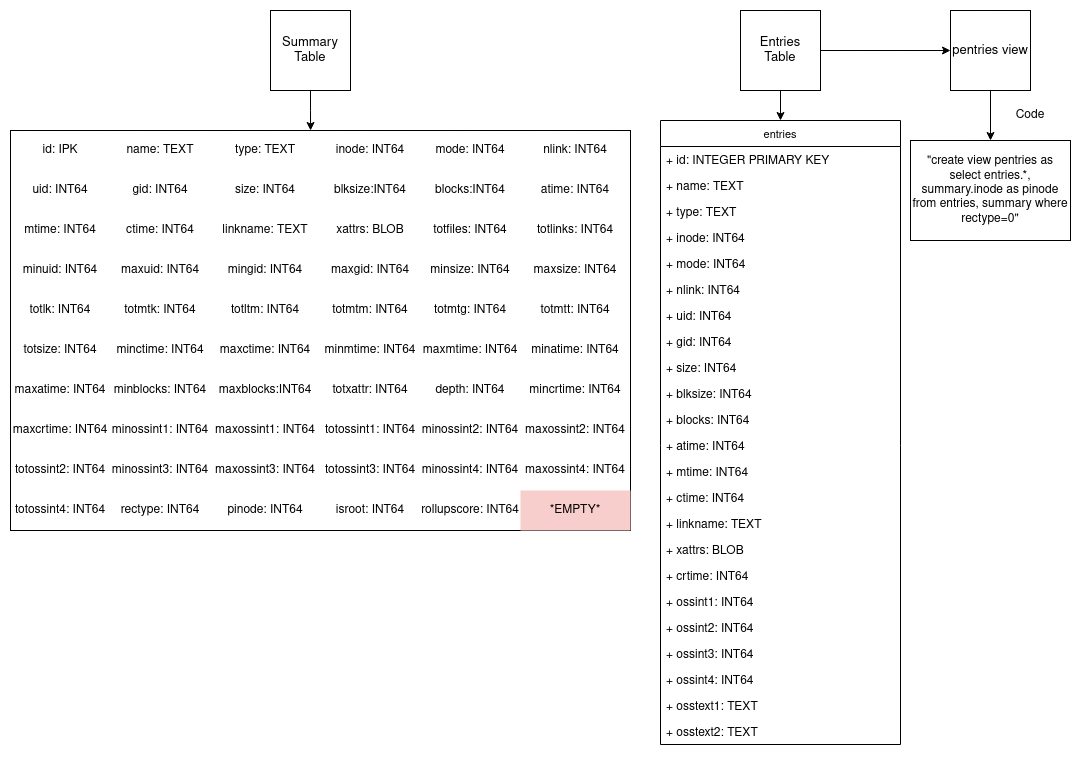
\includegraphics[width=1.0\textwidth]{images/Database_Schemas.png}
\caption{\label{fig:Database Schema}Database schema}
\end{figure}

\subsection{\pentries}
The original \pentries view was defined as:
\\\\
\texttt{SELECT entries.*, summary.inode FROM entries, summary};
\\\\
This was done in order to not store the parent inode of each entry,
which would be the same for every entry.

In general, users should query the \pentries view over the \entries
table in order to obtain complete sets of data to query on.

\subsubsection{\pentriesrollup}
In order to simplify rolling up indicies, the \pentries table was
modified to also union with the \pentriesrollup table, which contains
all child \pentries views copied into the current directory.

\subsection{\treesummary}
Similar to the directory \summary table, GUFI also provides
functionality to generate \treesummary tables. Instead of summarizing
only the data found in the entries table of the current directory, the
\treesummary table summarizes the contents of the entire subtree,
allowing for queries to completely skip processing entire subtries.

Generating \treesummary tables can be a very costly operation if done
on every single directory. Due to this, \treesummary tables are not
generated by default. Instead, they are generated by the \bfti
executable that must be run manually after indexing has completed.

\subsection{\vsummarydir}
The \vsummarydir view provides access to the entire directory summary
and not a partial directory summary (say by user or group).

\subsection{\vsummaryuser}
The \vsummaryuser view provides access to the directory summary for
each user (if this summary has been populated (not by default but
easily populatable via a query)).

\subsection{\vsummarygroup}
The \vsummarygroup view provides access to the directory summary for
each group (if this summary has been populated (not by default but
easily populatable via a query)).

\subsection{\vtsummarydir}
The vtsummarydir view provides access to the entire tree directory
summary and not a partial directory summary (say by user or group).

\subsection{\vtsummaryuser}
The \vtsummaryuser view provides access to the tree directory summary
for each user (if this summary has been populated (not by default but
easily populatable via a query)).

\subsection{\vtsummarygroup}
The \vtsummarygroup view provides access to the tree directory summary
for each group (if this summary has been populated (not by default but
easily populatable via a query)).

\subsection{\xattrs}
With the addition of extended attributes support, several more tables
and views were added into db.db. Additional database files with
different schemas were also added. See Section~\ref{sec:xattr_schema}
for details.

% This file is part of GUFI, which is part of MarFS, which is released
% under the BSD license.
%
%
% Copyright (c) 2017, Los Alamos National Security (LANS), LLC
% All rights reserved.
%
% Redistribution and use in source and binary forms, with or without modification,
% are permitted provided that the following conditions are met:
%
% 1. Redistributions of source code must retain the above copyright notice, this
% list of conditions and the following disclaimer.
%
% 2. Redistributions in binary form must reproduce the above copyright notice,
% this list of conditions and the following disclaimer in the documentation and/or
% other materials provided with the distribution.
%
% 3. Neither the name of the copyright holder nor the names of its contributors
% may be used to endorse or promote products derived from this software without
% specific prior written permission.
%
% THIS SOFTWARE IS PROVIDED BY THE COPYRIGHT HOLDERS AND CONTRIBUTORS "AS IS" AND
% ANY EXPRESS OR IMPLIED WARRANTIES, INCLUDING, BUT NOT LIMITED TO, THE IMPLIED
% WARRANTIES OF MERCHANTABILITY AND FITNESS FOR A PARTICULAR PURPOSE ARE DISCLAIMED.
% IN NO EVENT SHALL THE COPYRIGHT HOLDER OR CONTRIBUTORS BE LIABLE FOR ANY DIRECT,
% INDIRECT, INCIDENTAL, SPECIAL, EXEMPLARY, OR CONSEQUENTIAL DAMAGES (INCLUDING,
% BUT NOT LIMITED TO, PROCUREMENT OF SUBSTITUTE GOODS OR SERVICES; LOSS OF USE,
% DATA, OR PROFITS; OR BUSINESS INTERRUPTION) HOWEVER CAUSED AND ON ANY THEORY OF
% LIABILITY, WHETHER IN CONTRACT, STRICT LIABILITY, OR TORT (INCLUDING NEGLIGENCE
% OR OTHERWISE) ARISING IN ANY WAY OUT OF THE USE OF THIS SOFTWARE, EVEN IF
% ADVISED OF THE POSSIBILITY OF SUCH DAMAGE.
%
%
% From Los Alamos National Security, LLC:
% LA-CC-15-039
%
% Copyright (c) 2017, Los Alamos National Security, LLC All rights reserved.
% Copyright 2017. Los Alamos National Security, LLC. This software was produced
% under U.S. Government contract DE-AC52-06NA25396 for Los Alamos National
% Laboratory (LANL), which is operated by Los Alamos National Security, LLC for
% the U.S. Department of Energy. The U.S. Government has rights to use,
% reproduce, and distribute this software.  NEITHER THE GOVERNMENT NOR LOS
% ALAMOS NATIONAL SECURITY, LLC MAKES ANY WARRANTY, EXPRESS OR IMPLIED, OR
% ASSUMES ANY LIABILITY FOR THE USE OF THIS SOFTWARE.  If software is
% modified to produce derivative works, such modified software should be
% clearly marked, so as not to confuse it with the version available from
% LANL.
%
% THIS SOFTWARE IS PROVIDED BY LOS ALAMOS NATIONAL SECURITY, LLC AND CONTRIBUTORS
% "AS IS" AND ANY EXPRESS OR IMPLIED WARRANTIES, INCLUDING, BUT NOT LIMITED TO,
% THE IMPLIED WARRANTIES OF MERCHANTABILITY AND FITNESS FOR A PARTICULAR PURPOSE
% ARE DISCLAIMED. IN NO EVENT SHALL LOS ALAMOS NATIONAL SECURITY, LLC OR
% CONTRIBUTORS BE LIABLE FOR ANY DIRECT, INDIRECT, INCIDENTAL, SPECIAL,
% EXEMPLARY, OR CONSEQUENTIAL DAMAGES (INCLUDING, BUT NOT LIMITED TO, PROCUREMENT
% OF SUBSTITUTE GOODS OR SERVICES; LOSS OF USE, DATA, OR PROFITS; OR BUSINESS
% INTERRUPTION) HOWEVER CAUSED AND ON ANY THEORY OF LIABILITY, WHETHER IN
% CONTRACT, STRICT LIABILITY, OR TORT (INCLUDING NEGLIGENCE OR OTHERWISE) ARISING
% IN ANY WAY OUT OF THE USE OF THIS SOFTWARE, EVEN IF ADVISED OF THE POSSIBILITY
% OF SUCH DAMAGE.



\section{Indexing}
The first step to using GUFI is indexing a source filesystem.

An index created by GUFI retains the shape of the source filesystem:
directories that exist in the source filesystem also exist in the
index. If an administrator created the index, the directories will
also have the same access permissions, uid, and gid.

Indicies will not contain any of the files that the source filesystem
contained. Instead, all metadata extracted from a single directory of
the source filesystem will be placed into a single database file,
called db.db, in the cooresponding directory in the index. Each
database file will be created with a fixed schema that includes the
tables listed in Sections \ref{sec:schema} and
\ref{sec:xattr_schema}. Additional database files may be created if
extended attributes are extracted (see Section~\ref{sec:xattrs}).

\subsection{Directly Indexing a Filesystem}
% This file is part of GUFI, which is part of MarFS, which is released
% under the BSD license.
%
%
% Copyright (c) 2017, Los Alamos National Security (LANS), LLC
% All rights reserved.
%
% Redistribution and use in source and binary forms, with or without modification,
% are permitted provided that the following conditions are met:
%
% 1. Redistributions of source code must retain the above copyright notice, this
% list of conditions and the following disclaimer.
%
% 2. Redistributions in binary form must reproduce the above copyright notice,
% this list of conditions and the following disclaimer in the documentation and/or
% other materials provided with the distribution.
%
% 3. Neither the name of the copyright holder nor the names of its contributors
% may be used to endorse or promote products derived from this software without
% specific prior written permission.
%
% THIS SOFTWARE IS PROVIDED BY THE COPYRIGHT HOLDERS AND CONTRIBUTORS "AS IS" AND
% ANY EXPRESS OR IMPLIED WARRANTIES, INCLUDING, BUT NOT LIMITED TO, THE IMPLIED
% WARRANTIES OF MERCHANTABILITY AND FITNESS FOR A PARTICULAR PURPOSE ARE DISCLAIMED.
% IN NO EVENT SHALL THE COPYRIGHT HOLDER OR CONTRIBUTORS BE LIABLE FOR ANY DIRECT,
% INDIRECT, INCIDENTAL, SPECIAL, EXEMPLARY, OR CONSEQUENTIAL DAMAGES (INCLUDING,
% BUT NOT LIMITED TO, PROCUREMENT OF SUBSTITUTE GOODS OR SERVICES; LOSS OF USE,
% DATA, OR PROFITS; OR BUSINESS INTERRUPTION) HOWEVER CAUSED AND ON ANY THEORY OF
% LIABILITY, WHETHER IN CONTRACT, STRICT LIABILITY, OR TORT (INCLUDING NEGLIGENCE
% OR OTHERWISE) ARISING IN ANY WAY OUT OF THE USE OF THIS SOFTWARE, EVEN IF
% ADVISED OF THE POSSIBILITY OF SUCH DAMAGE.
%
%
% From Los Alamos National Security, LLC:
% LA-CC-15-039
%
% Copyright (c) 2017, Los Alamos National Security, LLC All rights reserved.
% Copyright 2017. Los Alamos National Security, LLC. This software was produced
% under U.S. Government contract DE-AC52-06NA25396 for Los Alamos National
% Laboratory (LANL), which is operated by Los Alamos National Security, LLC for
% the U.S. Department of Energy. The U.S. Government has rights to use,
% reproduce, and distribute this software.  NEITHER THE GOVERNMENT NOR LOS
% ALAMOS NATIONAL SECURITY, LLC MAKES ANY WARRANTY, EXPRESS OR IMPLIED, OR
% ASSUMES ANY LIABILITY FOR THE USE OF THIS SOFTWARE.  If software is
% modified to produce derivative works, such modified software should be
% clearly marked, so as not to confuse it with the version available from
% LANL.
%
% THIS SOFTWARE IS PROVIDED BY LOS ALAMOS NATIONAL SECURITY, LLC AND CONTRIBUTORS
% "AS IS" AND ANY EXPRESS OR IMPLIED WARRANTIES, INCLUDING, BUT NOT LIMITED TO,
% THE IMPLIED WARRANTIES OF MERCHANTABILITY AND FITNESS FOR A PARTICULAR PURPOSE
% ARE DISCLAIMED. IN NO EVENT SHALL LOS ALAMOS NATIONAL SECURITY, LLC OR
% CONTRIBUTORS BE LIABLE FOR ANY DIRECT, INDIRECT, INCIDENTAL, SPECIAL,
% EXEMPLARY, OR CONSEQUENTIAL DAMAGES (INCLUDING, BUT NOT LIMITED TO, PROCUREMENT
% OF SUBSTITUTE GOODS OR SERVICES; LOSS OF USE, DATA, OR PROFITS; OR BUSINESS
% INTERRUPTION) HOWEVER CAUSED AND ON ANY THEORY OF LIABILITY, WHETHER IN
% CONTRACT, STRICT LIABILITY, OR TORT (INCLUDING NEGLIGENCE OR OTHERWISE) ARISING
% IN ANY WAY OUT OF THE USE OF THIS SOFTWARE, EVEN IF ADVISED OF THE POSSIBILITY
% OF SUCH DAMAGE.



\section{gufi\_dir2index}
\gufidirindex is used in order to directly create an index based off
of the contents of a provided directory.

\subsubsection{Database Templates}
One optimization made to \gufidirindex was the creation of a database
template file. Instead of creating new databases via SQLite in every
single directory, the template is copied into each directory as a
bytestream. This avoids checks done by SQLite when setting up databases.

\subsection{Flags}

\begin{table} [h]
  \centering
  \begin{tabular}{l|r}
    Flag & Functionality \\\hline
    -h & help manual \\
    -H & Show assigned input values \\
    -n \textless num\_threads\textgreater  & define number of threads to use \\
    -x & pull xattrs from source file-sys into GUFI \\
    -z \textless max\_level\textgreater & maximum level to go down to
  \end{tabular}
  \caption{\label{fig:Flags_for_dir2index} \gufidirindex Flags and Arguments}
\end{table}

\begin{figure} [h]
  \centering
  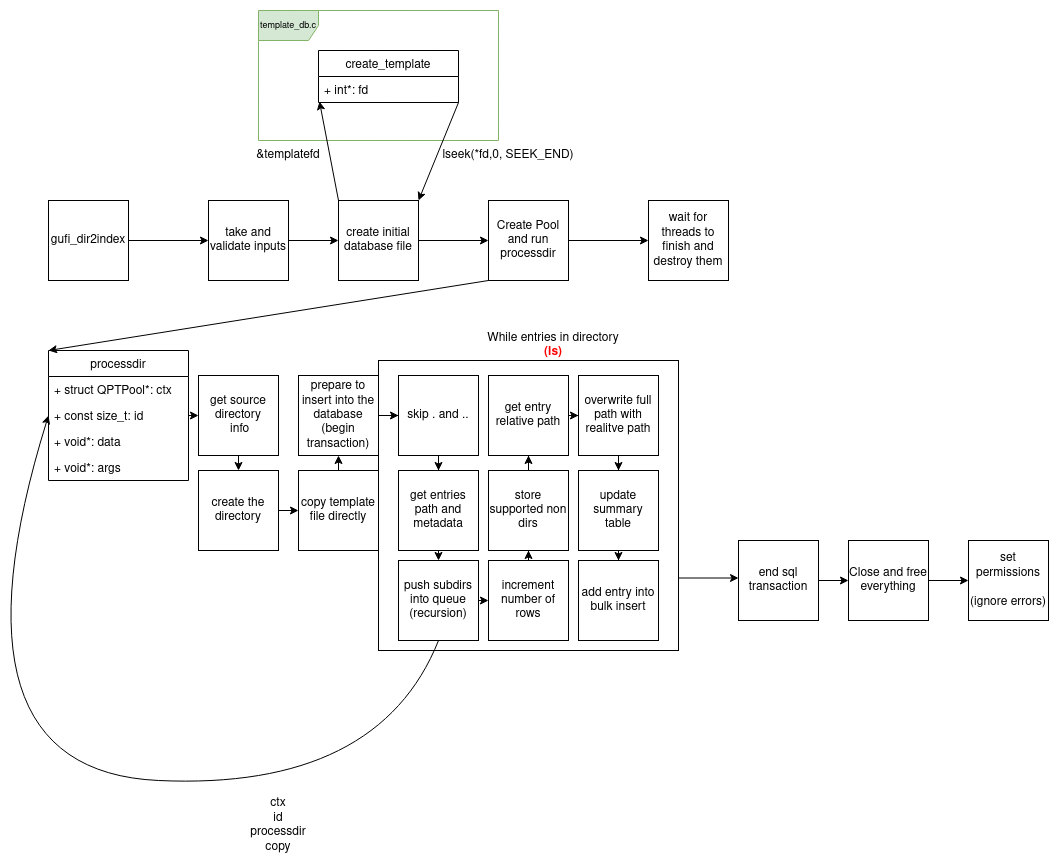
\includegraphics[width=1.0\textwidth]{images/gufi_dir2index.png}
  \caption{\label{fig:gufi_dir2index} \gufidirindex workflow}
\end{figure}

\subsection{Usage}
\gufidirindex \texttt{[flags] [directory to index] [location to place indexed directory]}

\subsection{Indirectly Indexing a Filesystem}
% This file is part of GUFI, which is part of MarFS, which is released
% under the BSD license.
%
%
% Copyright (c) 2017, Los Alamos National Security (LANS), LLC
% All rights reserved.
%
% Redistribution and use in source and binary forms, with or without modification,
% are permitted provided that the following conditions are met:
%
% 1. Redistributions of source code must retain the above copyright notice, this
% list of conditions and the following disclaimer.
%
% 2. Redistributions in binary form must reproduce the above copyright notice,
% this list of conditions and the following disclaimer in the documentation and/or
% other materials provided with the distribution.
%
% 3. Neither the name of the copyright holder nor the names of its contributors
% may be used to endorse or promote products derived from this software without
% specific prior written permission.
%
% THIS SOFTWARE IS PROVIDED BY THE COPYRIGHT HOLDERS AND CONTRIBUTORS "AS IS" AND
% ANY EXPRESS OR IMPLIED WARRANTIES, INCLUDING, BUT NOT LIMITED TO, THE IMPLIED
% WARRANTIES OF MERCHANTABILITY AND FITNESS FOR A PARTICULAR PURPOSE ARE DISCLAIMED.
% IN NO EVENT SHALL THE COPYRIGHT HOLDER OR CONTRIBUTORS BE LIABLE FOR ANY DIRECT,
% INDIRECT, INCIDENTAL, SPECIAL, EXEMPLARY, OR CONSEQUENTIAL DAMAGES (INCLUDING,
% BUT NOT LIMITED TO, PROCUREMENT OF SUBSTITUTE GOODS OR SERVICES; LOSS OF USE,
% DATA, OR PROFITS; OR BUSINESS INTERRUPTION) HOWEVER CAUSED AND ON ANY THEORY OF
% LIABILITY, WHETHER IN CONTRACT, STRICT LIABILITY, OR TORT (INCLUDING NEGLIGENCE
% OR OTHERWISE) ARISING IN ANY WAY OUT OF THE USE OF THIS SOFTWARE, EVEN IF
% ADVISED OF THE POSSIBILITY OF SUCH DAMAGE.
%
%
% From Los Alamos National Security, LLC:
% LA-CC-15-039
%
% Copyright (c) 2017, Los Alamos National Security, LLC All rights reserved.
% Copyright 2017. Los Alamos National Security, LLC. This software was produced
% under U.S. Government contract DE-AC52-06NA25396 for Los Alamos National
% Laboratory (LANL), which is operated by Los Alamos National Security, LLC for
% the U.S. Department of Energy. The U.S. Government has rights to use,
% reproduce, and distribute this software.  NEITHER THE GOVERNMENT NOR LOS
% ALAMOS NATIONAL SECURITY, LLC MAKES ANY WARRANTY, EXPRESS OR IMPLIED, OR
% ASSUMES ANY LIABILITY FOR THE USE OF THIS SOFTWARE.  If software is
% modified to produce derivative works, such modified software should be
% clearly marked, so as not to confuse it with the version available from
% LANL.
%
% THIS SOFTWARE IS PROVIDED BY LOS ALAMOS NATIONAL SECURITY, LLC AND CONTRIBUTORS
% "AS IS" AND ANY EXPRESS OR IMPLIED WARRANTIES, INCLUDING, BUT NOT LIMITED TO,
% THE IMPLIED WARRANTIES OF MERCHANTABILITY AND FITNESS FOR A PARTICULAR PURPOSE
% ARE DISCLAIMED. IN NO EVENT SHALL LOS ALAMOS NATIONAL SECURITY, LLC OR
% CONTRIBUTORS BE LIABLE FOR ANY DIRECT, INDIRECT, INCIDENTAL, SPECIAL,
% EXEMPLARY, OR CONSEQUENTIAL DAMAGES (INCLUDING, BUT NOT LIMITED TO, PROCUREMENT
% OF SUBSTITUTE GOODS OR SERVICES; LOSS OF USE, DATA, OR PROFITS; OR BUSINESS
% INTERRUPTION) HOWEVER CAUSED AND ON ANY THEORY OF LIABILITY, WHETHER IN
% CONTRACT, STRICT LIABILITY, OR TORT (INCLUDING NEGLIGENCE OR OTHERWISE) ARISING
% IN ANY WAY OUT OF THE USE OF THIS SOFTWARE, EVEN IF ADVISED OF THE POSSIBILITY
% OF SUCH DAMAGE.



\subsubsection{Trace Files}
\label{sec:tracefiles}
Traces files, or flat files, are text files containing \lstat
information pulled from source filesystems separated by
delimiters. Trace files are generated by \gufidirtrace and are
processed by \gufitraceindex.

The default delimiter is the ASCII Record Separator character
\texttt{\textbackslash x1E}, but can be changed to any 8-bit
character. Characters that can appear in filesystems should not be
used as the delimiter in order to not confuse \gufitraceindex.

The metadata pulled from each directory is represented by a ``stanza''
in a trace file. A stanza starts with a line of directory metadata
followed by zero or more lines of regular file and symbolic link
metadata. Note that the summary of each directory is not stored in
trace files and are instead generated when the index is built.

Due to the parallelism of indexing, stanzas can appear in any order
within a trace file and can be placed in any of the per thread trace
files that are generated. Traces files can be concatenated together if
doing so is necessary or more convenient.

\section{gufi\_dir2trace}
gufi\_dir2trace is to generate a trace of the files and directories inside of a specified root directory
\subsection{Flags}

\begin{table} [h]
\centering
\begin{tabular}{l|r}
Flag & Functionality \\\hline
-h & help manual \\
-H & Show assigned input values \\
-n \textless num\_threads\textgreater  & define number of threads to use \\
-x & pull xattrs from source file-sys into GUFI \\
-z \textless max\_level\textgreater & maximum level to go down to
\end{tabular}
\caption{\label{fig:Flags_for_dir2trace}gufi\_dir2trace Flags and Arguments}
\end{table}

\subsection{Usage}
\texttt{gufi\_dir2trace [flags] [directory to trace] [prefix of output files]}
% This file is part of GUFI, which is part of MarFS, which is released
% under the BSD license.
%
%
% Copyright (c) 2017, Los Alamos National Security (LANS), LLC
% All rights reserved.
%
% Redistribution and use in source and binary forms, with or without modification,
% are permitted provided that the following conditions are met:
%
% 1. Redistributions of source code must retain the above copyright notice, this
% list of conditions and the following disclaimer.
%
% 2. Redistributions in binary form must reproduce the above copyright notice,
% this list of conditions and the following disclaimer in the documentation and/or
% other materials provided with the distribution.
%
% 3. Neither the name of the copyright holder nor the names of its contributors
% may be used to endorse or promote products derived from this software without
% specific prior written permission.
%
% THIS SOFTWARE IS PROVIDED BY THE COPYRIGHT HOLDERS AND CONTRIBUTORS "AS IS" AND
% ANY EXPRESS OR IMPLIED WARRANTIES, INCLUDING, BUT NOT LIMITED TO, THE IMPLIED
% WARRANTIES OF MERCHANTABILITY AND FITNESS FOR A PARTICULAR PURPOSE ARE DISCLAIMED.
% IN NO EVENT SHALL THE COPYRIGHT HOLDER OR CONTRIBUTORS BE LIABLE FOR ANY DIRECT,
% INDIRECT, INCIDENTAL, SPECIAL, EXEMPLARY, OR CONSEQUENTIAL DAMAGES (INCLUDING,
% BUT NOT LIMITED TO, PROCUREMENT OF SUBSTITUTE GOODS OR SERVICES; LOSS OF USE,
% DATA, OR PROFITS; OR BUSINESS INTERRUPTION) HOWEVER CAUSED AND ON ANY THEORY OF
% LIABILITY, WHETHER IN CONTRACT, STRICT LIABILITY, OR TORT (INCLUDING NEGLIGENCE
% OR OTHERWISE) ARISING IN ANY WAY OUT OF THE USE OF THIS SOFTWARE, EVEN IF
% ADVISED OF THE POSSIBILITY OF SUCH DAMAGE.
%
%
% From Los Alamos National Security, LLC:
% LA-CC-15-039
%
% Copyright (c) 2017, Los Alamos National Security, LLC All rights reserved.
% Copyright 2017. Los Alamos National Security, LLC. This software was produced
% under U.S. Government contract DE-AC52-06NA25396 for Los Alamos National
% Laboratory (LANL), which is operated by Los Alamos National Security, LLC for
% the U.S. Department of Energy. The U.S. Government has rights to use,
% reproduce, and distribute this software.  NEITHER THE GOVERNMENT NOR LOS
% ALAMOS NATIONAL SECURITY, LLC MAKES ANY WARRANTY, EXPRESS OR IMPLIED, OR
% ASSUMES ANY LIABILITY FOR THE USE OF THIS SOFTWARE.  If software is
% modified to produce derivative works, such modified software should be
% clearly marked, so as not to confuse it with the version available from
% LANL.
%
% THIS SOFTWARE IS PROVIDED BY LOS ALAMOS NATIONAL SECURITY, LLC AND CONTRIBUTORS
% "AS IS" AND ANY EXPRESS OR IMPLIED WARRANTIES, INCLUDING, BUT NOT LIMITED TO,
% THE IMPLIED WARRANTIES OF MERCHANTABILITY AND FITNESS FOR A PARTICULAR PURPOSE
% ARE DISCLAIMED. IN NO EVENT SHALL LOS ALAMOS NATIONAL SECURITY, LLC OR
% CONTRIBUTORS BE LIABLE FOR ANY DIRECT, INDIRECT, INCIDENTAL, SPECIAL,
% EXEMPLARY, OR CONSEQUENTIAL DAMAGES (INCLUDING, BUT NOT LIMITED TO, PROCUREMENT
% OF SUBSTITUTE GOODS OR SERVICES; LOSS OF USE, DATA, OR PROFITS; OR BUSINESS
% INTERRUPTION) HOWEVER CAUSED AND ON ANY THEORY OF LIABILITY, WHETHER IN
% CONTRACT, STRICT LIABILITY, OR TORT (INCLUDING NEGLIGENCE OR OTHERWISE) ARISING
% IN ANY WAY OUT OF THE USE OF THIS SOFTWARE, EVEN IF ADVISED OF THE POSSIBILITY
% OF SUCH DAMAGE.



\subsubsection{\gufitraceindex}
\gufitraceindex is used to convert trace files into indicies. It is
essentially the same as \gufidirindex except it obtains data from
trace files instead of the filesystem being indexed.

Per thread trace files may be passed into \gufitraceindex
directly. Note that passing in too many trace files at once might
result in running out of file descriptors. Alternatively, the per
thread trace files may be concatenated in any order into a smaller
number of larger files for processing.

\paragraph{\texttt{scout\_function}} ~\\
One important design decision made to \gufitraceindex was the
implementation of a thread to find the starting offsets of stanzas
from the input trace file and {\it not} process the stanza. Instead,
the starting offsets are enqueued in the thread pool and processed
concurrently with the scouting thread.

\paragraph{Usage} ~\\
\gufitraceindex \texttt{[flags] trace\_file [trace\_file ...] index\_root}

% This file is part of GUFI, which is part of MarFS, which is released
% under the BSD license.
%
%
% Copyright (c) 2017, Los Alamos National Security (LANS), LLC
% All rights reserved.
%
% Redistribution and use in source and binary forms, with or without modification,
% are permitted provided that the following conditions are met:
%
% 1. Redistributions of source code must retain the above copyright notice, this
% list of conditions and the following disclaimer.
%
% 2. Redistributions in binary form must reproduce the above copyright notice,
% this list of conditions and the following disclaimer in the documentation and/or
% other materials provided with the distribution.
%
% 3. Neither the name of the copyright holder nor the names of its contributors
% may be used to endorse or promote products derived from this software without
% specific prior written permission.
%
% THIS SOFTWARE IS PROVIDED BY THE COPYRIGHT HOLDERS AND CONTRIBUTORS "AS IS" AND
% ANY EXPRESS OR IMPLIED WARRANTIES, INCLUDING, BUT NOT LIMITED TO, THE IMPLIED
% WARRANTIES OF MERCHANTABILITY AND FITNESS FOR A PARTICULAR PURPOSE ARE DISCLAIMED.
% IN NO EVENT SHALL THE COPYRIGHT HOLDER OR CONTRIBUTORS BE LIABLE FOR ANY DIRECT,
% INDIRECT, INCIDENTAL, SPECIAL, EXEMPLARY, OR CONSEQUENTIAL DAMAGES (INCLUDING,
% BUT NOT LIMITED TO, PROCUREMENT OF SUBSTITUTE GOODS OR SERVICES; LOSS OF USE,
% DATA, OR PROFITS; OR BUSINESS INTERRUPTION) HOWEVER CAUSED AND ON ANY THEORY OF
% LIABILITY, WHETHER IN CONTRACT, STRICT LIABILITY, OR TORT (INCLUDING NEGLIGENCE
% OR OTHERWISE) ARISING IN ANY WAY OUT OF THE USE OF THIS SOFTWARE, EVEN IF
% ADVISED OF THE POSSIBILITY OF SUCH DAMAGE.
%
%
% From Los Alamos National Security, LLC:
% LA-CC-15-039
%
% Copyright (c) 2017, Los Alamos National Security, LLC All rights reserved.
% Copyright 2017. Los Alamos National Security, LLC. This software was produced
% under U.S. Government contract DE-AC52-06NA25396 for Los Alamos National
% Laboratory (LANL), which is operated by Los Alamos National Security, LLC for
% the U.S. Department of Energy. The U.S. Government has rights to use,
% reproduce, and distribute this software.  NEITHER THE GOVERNMENT NOR LOS
% ALAMOS NATIONAL SECURITY, LLC MAKES ANY WARRANTY, EXPRESS OR IMPLIED, OR
% ASSUMES ANY LIABILITY FOR THE USE OF THIS SOFTWARE.  If software is
% modified to produce derivative works, such modified software should be
% clearly marked, so as not to confuse it with the version available from
% LANL.
%
% THIS SOFTWARE IS PROVIDED BY LOS ALAMOS NATIONAL SECURITY, LLC AND CONTRIBUTORS
% "AS IS" AND ANY EXPRESS OR IMPLIED WARRANTIES, INCLUDING, BUT NOT LIMITED TO,
% THE IMPLIED WARRANTIES OF MERCHANTABILITY AND FITNESS FOR A PARTICULAR PURPOSE
% ARE DISCLAIMED. IN NO EVENT SHALL LOS ALAMOS NATIONAL SECURITY, LLC OR
% CONTRIBUTORS BE LIABLE FOR ANY DIRECT, INDIRECT, INCIDENTAL, SPECIAL,
% EXEMPLARY, OR CONSEQUENTIAL DAMAGES (INCLUDING, BUT NOT LIMITED TO, PROCUREMENT
% OF SUBSTITUTE GOODS OR SERVICES; LOSS OF USE, DATA, OR PROFITS; OR BUSINESS
% INTERRUPTION) HOWEVER CAUSED AND ON ANY THEORY OF LIABILITY, WHETHER IN
% CONTRACT, STRICT LIABILITY, OR TORT (INCLUDING NEGLIGENCE OR OTHERWISE) ARISING
% IN ANY WAY OUT OF THE USE OF THIS SOFTWARE, EVEN IF ADVISED OF THE POSSIBILITY
% OF SUCH DAMAGE.



\section{Extended Attributes}
\label{sec:xattrs}
GUFI supports the indexing and querying of user data through extended
attributes (xattrs).

Reading standard filesystem permissions of files only requires read
(and execute) access to the directory. Extended attribute names are
visible this way. However, because xattr values are user defined data,
their permissions are checked at the file level, requiring changes to
how GUFI stores data. For more information on xattrs, see
\texttt{xattr(7)}, \listxattr, and \getxattr.

\subsection{Indexing}
Directories containing files from multiple users might have xattrs
that are not readable by all who can view the \lstat data of the
directory. As GUFI was originally designed to only use directory-level
permission checks, a number of modifications were made to process
xattrs without violating their permissions.

\subsubsection{Roll In Rules}
Xattrs that are readable by all who have access to the directory are
stored in the \xattrspwd table in the main database. These xattrs are
referred to as ``rolled in''.

The rules that determine whether or not an xattr pair can roll in are
as follows:

\begin{itemize}
\item File is 0+R
\item File is UG+R doesnt matter on other, with file and parent same
  usr and grp and parent has only UG+R with no other read
\item File is U+R doesnt matter on grp and other, with file and parent
  same usr and parent dir has only U+R, no grp and other read
\item Directory has write for every read:
    \texttt{drw*rw*rw*} or \texttt{drw*rw*\_\_\_} or
    \texttt{drw*\_\_\_\_\_\_} - if you can write the dir you can
    chmod the files to see the xattrs
\end{itemize}

Xattrs that cannot be read by all who can read the directory are
stored in external per-uid and per-gid databases set with
\texttt{uid:nobody} and \texttt{nobody:gid} owners respectively. This
makes it so that non-admin users cannot access the xattrs stored in
external databases that they do not have permissions to access.

\subsubsection{Schema}
\label{sec:xattr_schema}
The main database and all external databases contain the following
tables and views:

\begin{itemize}
\item The \xattrspwd table contains all extended attributes of the
  current directory that were placed into this database file.

\item The \xattrsrollup table contains all extended attributes that
  were placed into the children directories that were subsequently
  rolled up into the current directory.

\item The \xattrsavail view is the union of all extended attributes
  in \xattrspwd and \xattrsrollup in this database file.
\end{itemize}

Additionally, each main database file has the following tables and
views in order to keep track of which files were created by GUFI for
the purposes of storing xattrs:

\begin{itemize}
\item The \xattrfilespwd table contains a listing of external database
  filenames that contain xattrs that were not rolled in.
\item The \xattrfilesrollup table contains a listing of external
  database filenames that contain xattrs that were not
  rolled in, but were brought in by rolling up.
\item The \xattrfiles view combines the listings of database filenames
  found in \xattrfilespwd and \xattrfilesrollup.
\end{itemize}

\subsubsection{Usage}
Extended attributes are not pulled from the filesystem by default. In
order to pull them, pass \texttt{-x} to \gufidirindex or
\gufidirtrace.

Note that only xattr pairs in the user namespace (\texttt{user.*}) are
extracted.

\subsubsection{Rollup}
Additional steps were added to rollups in order to copy rolled up
xattrs upwards properly:

\begin{itemize}
\item The child's \xattrsavail view (without external database data)
  is copied into the parent's \xattrsrollup table.
\item The child's \xattrfiles view (without external databases data)
  is copied into the parent's \xattrfilesrollup table.
\item The child's external database files are copied into the
  parent. If the parent already has an external database file with the
  same uid or gid, the contents of the external database are copied
  into the parent's external database's \xattrsrollup table instead.
\end{itemize}

\subsection{Querying}
When querying for xattrs, pass \texttt{-x} to \gufiquery to build the
\xattrs view for querying. This view is a SQL union of rolled in
xattrs and any external databases that successfully
attaches. Attaching the database files checks the permissions of the
xattrs. \texttt{UNION} removes duplicate entries that showed up in
multiple external databases, leaving a unique set of xattrs accessible
by the caller.

The \xentries, \xpentries, \xsummary views are convenience views
generated so that users do not have to perform joins themselves. Like
the \xattrs view, these views are also dropped at the end of directory
processing.

Note that entries with multiple extended attributes will return
multiple times in this view.


\subsection{Location}
GUFI is expected to be used to query the indices of many filesystems
all at once. However, the source filesystems are not expected to be
accessible from each other. In order for the indices from many
disconnected systems to be queried at once, they should all be built
under a common directory on a single machine.

\subsubsection{Permissions}
If a GUFI index is located on a different machine than the source
tree, the users and groups are probably not available on the machine
with the index on it. \texttt{/etc/passwd} should be populated with
the entries from the source machine and modified so that they do not
have a home directory, and are not allowed to log in
(\texttt{/sbin/nologin}). Similarly, \texttt{/etc/group} should be
updated with the source machine's groups and modified to remove any
unnecessary information.

% This file is part of GUFI, which is part of MarFS, which is released
% under the BSD license.
%
%
% Copyright (c) 2017, Los Alamos National Security (LANS), LLC
% All rights reserved.
%
% Redistribution and use in source and binary forms, with or without modification,
% are permitted provided that the following conditions are met:
%
% 1. Redistributions of source code must retain the above copyright notice, this
% list of conditions and the following disclaimer.
%
% 2. Redistributions in binary form must reproduce the above copyright notice,
% this list of conditions and the following disclaimer in the documentation and/or
% other materials provided with the distribution.
%
% 3. Neither the name of the copyright holder nor the names of its contributors
% may be used to endorse or promote products derived from this software without
% specific prior written permission.
%
% THIS SOFTWARE IS PROVIDED BY THE COPYRIGHT HOLDERS AND CONTRIBUTORS "AS IS" AND
% ANY EXPRESS OR IMPLIED WARRANTIES, INCLUDING, BUT NOT LIMITED TO, THE IMPLIED
% WARRANTIES OF MERCHANTABILITY AND FITNESS FOR A PARTICULAR PURPOSE ARE DISCLAIMED.
% IN NO EVENT SHALL THE COPYRIGHT HOLDER OR CONTRIBUTORS BE LIABLE FOR ANY DIRECT,
% INDIRECT, INCIDENTAL, SPECIAL, EXEMPLARY, OR CONSEQUENTIAL DAMAGES (INCLUDING,
% BUT NOT LIMITED TO, PROCUREMENT OF SUBSTITUTE GOODS OR SERVICES; LOSS OF USE,
% DATA, OR PROFITS; OR BUSINESS INTERRUPTION) HOWEVER CAUSED AND ON ANY THEORY OF
% LIABILITY, WHETHER IN CONTRACT, STRICT LIABILITY, OR TORT (INCLUDING NEGLIGENCE
% OR OTHERWISE) ARISING IN ANY WAY OUT OF THE USE OF THIS SOFTWARE, EVEN IF
% ADVISED OF THE POSSIBILITY OF SUCH DAMAGE.
%
%
% From Los Alamos National Security, LLC:
% LA-CC-15-039
%
% Copyright (c) 2017, Los Alamos National Security, LLC All rights reserved.
% Copyright 2017. Los Alamos National Security, LLC. This software was produced
% under U.S. Government contract DE-AC52-06NA25396 for Los Alamos National
% Laboratory (LANL), which is operated by Los Alamos National Security, LLC for
% the U.S. Department of Energy. The U.S. Government has rights to use,
% reproduce, and distribute this software.  NEITHER THE GOVERNMENT NOR LOS
% ALAMOS NATIONAL SECURITY, LLC MAKES ANY WARRANTY, EXPRESS OR IMPLIED, OR
% ASSUMES ANY LIABILITY FOR THE USE OF THIS SOFTWARE.  If software is
% modified to produce derivative works, such modified software should be
% clearly marked, so as not to confuse it with the version available from
% LANL.
%
% THIS SOFTWARE IS PROVIDED BY LOS ALAMOS NATIONAL SECURITY, LLC AND CONTRIBUTORS
% "AS IS" AND ANY EXPRESS OR IMPLIED WARRANTIES, INCLUDING, BUT NOT LIMITED TO,
% THE IMPLIED WARRANTIES OF MERCHANTABILITY AND FITNESS FOR A PARTICULAR PURPOSE
% ARE DISCLAIMED. IN NO EVENT SHALL LOS ALAMOS NATIONAL SECURITY, LLC OR
% CONTRIBUTORS BE LIABLE FOR ANY DIRECT, INDIRECT, INCIDENTAL, SPECIAL,
% EXEMPLARY, OR CONSEQUENTIAL DAMAGES (INCLUDING, BUT NOT LIMITED TO, PROCUREMENT
% OF SUBSTITUTE GOODS OR SERVICES; LOSS OF USE, DATA, OR PROFITS; OR BUSINESS
% INTERRUPTION) HOWEVER CAUSED AND ON ANY THEORY OF LIABILITY, WHETHER IN
% CONTRACT, STRICT LIABILITY, OR TORT (INCLUDING NEGLIGENCE OR OTHERWISE) ARISING
% IN ANY WAY OUT OF THE USE OF THIS SOFTWARE, EVEN IF ADVISED OF THE POSSIBILITY
% OF SUCH DAMAGE.



\section{Rollup}
\label{sec:rollup}
After an index is created, the index may be rolled up. Rolling up is a
major optimization that can reduce the number of directories that need
to be opened when querying by significant amounts while still
obtaining the same results as an unmodified index.

\subsection{Bottlenecks}
During querying, every single directory runs a fixed set of
operations:

\begin{itemize}
  \item \texttt{opendir(3)}
  \item \texttt{readdir(3)} (Looped)
  \item \texttt{sqlite3\_open\_v2}
  \item \texttt{sqlite3\_exec\_v2}
  \item \texttt{sqlite3\_close(3)}
  \item \texttt{closedir(3)}
\end{itemize}

Each of these operations have costs associated with them. Some are
fixed and some depend on the shape and contents of the index. Reducing
the number of directories processed allows for fixed costs to be
amortized.

\subsection{Rules}
\label{rolluprules}
\subsubsection{Whether or not a directory {\it CAN} roll up}
In order for a child directory to be allowed to roll up into its
parent directory, it must follow two rules. First, all of its children
must be rolled up. Second, all of its children must have permissions
that satisfy any one of the following conditions with the parent.

\begin{itemize}
  \item World readable and executable (o+rx)
  \item Matching user, group, and others permissions, with the same
    user and group
  \item Matching user and group permissions, readable and executable
    (ug+rx) with the same user and group, and not world readable and
    excutable (o-rx)
  \item Matching user permissions, readable and executable (u+rx) with
    the same user and not group or world readable and executable
    (go-rx)
\end{itemize}

Note that because leaf directories have no children with which to have
conflicting permission with, they are considered rolled up.

\subsubsection{Whether or not a directory {\it SHOULD} roll up}
In addition to the permission-based rules that determine whether or
not a directory can roll up, we also have a small check to say whether
or not a directory should roll up.

As data is rolled upwards in the index, databases towards the top will
accumulate more and more data from its subtrees. If directories are
allowed to roll up without limit, some databases will become
significantly larger than others, causing large amounts of tail
latency.

The \rollup executable has the \texttt{-L} flag that limits the number
of entries that may be found within a single directory.

\subsection{Steps}
The processing of rolling up involves a number of steps that update
the tables of the parent directory.

First, the target directory is checked to ensure it can and should
roll up its children into itself using the rules listed in
\ref{rolluprules}. If rollup will proceed, the parent's \summary table
is updated with a rollup score of 1.

Then, the contents each child is copied into the parent:

\begin{enumerate}
\item The child's \pentries view is copied into the parent's
  \pentriesrollup table. The parent's \pentries view is updated
  automatically.
\item The child's \summary table is copied into the parent's \summary
  table with the names of each child directory prefixed with the parent's
  name.
\end{enumerate}

Rolling up can be viewed as flattening the contents of the index while
taking into consideration the permissions of each directory.

Rolling up will cause the size of the index to grow significantly due
to the amount of data being replicated. One obvious optimization would
be to only roll up to the top-most level where a directory can roll up
to (one extra copy of the subtree instead of repeated copies). This
however, will only allow for queries to take advantage of rollups if
they start above the top-most rollup directory. Starting a query below
the top-most rollup level would result in the original subtree's query
time whereas the implemented method of rolling up allows for queries
starting at any point in the index to take advantage of rollups.

The rollup operation can take some time, and so indicies are not
rolled up automatically. The \rollup executable must be called
manually.

\subsection{Querying}
Prior to rolling up, the \pentries view can be treated as an optional
improvement to the \entries table. After rolling up, the \pentries view
will have been updated extensively and should always be used when
querying rolled up indicies. Querying the \entries table will return
only the entries found in the directories that were processed.

\subsection{\rollup executable}
In order to apply rollup to an index, run the \rollup executable:
\\\\
\indent \rollup \texttt{[index root]}
\\\\
Figure~\ref{fig:rollupworkflow} shows the overall structure of the \rollup
executable. The \rollup executable uses the BottomUp code (see
Section~\ref{sec:bottomup}) to recursively descend the original index and only
perform the rollup operation once all children have been processed as
shown in Figure~\ref{fig:rollupfunction}.

\begin{sidewaysfigure} [!htb]
  \centering 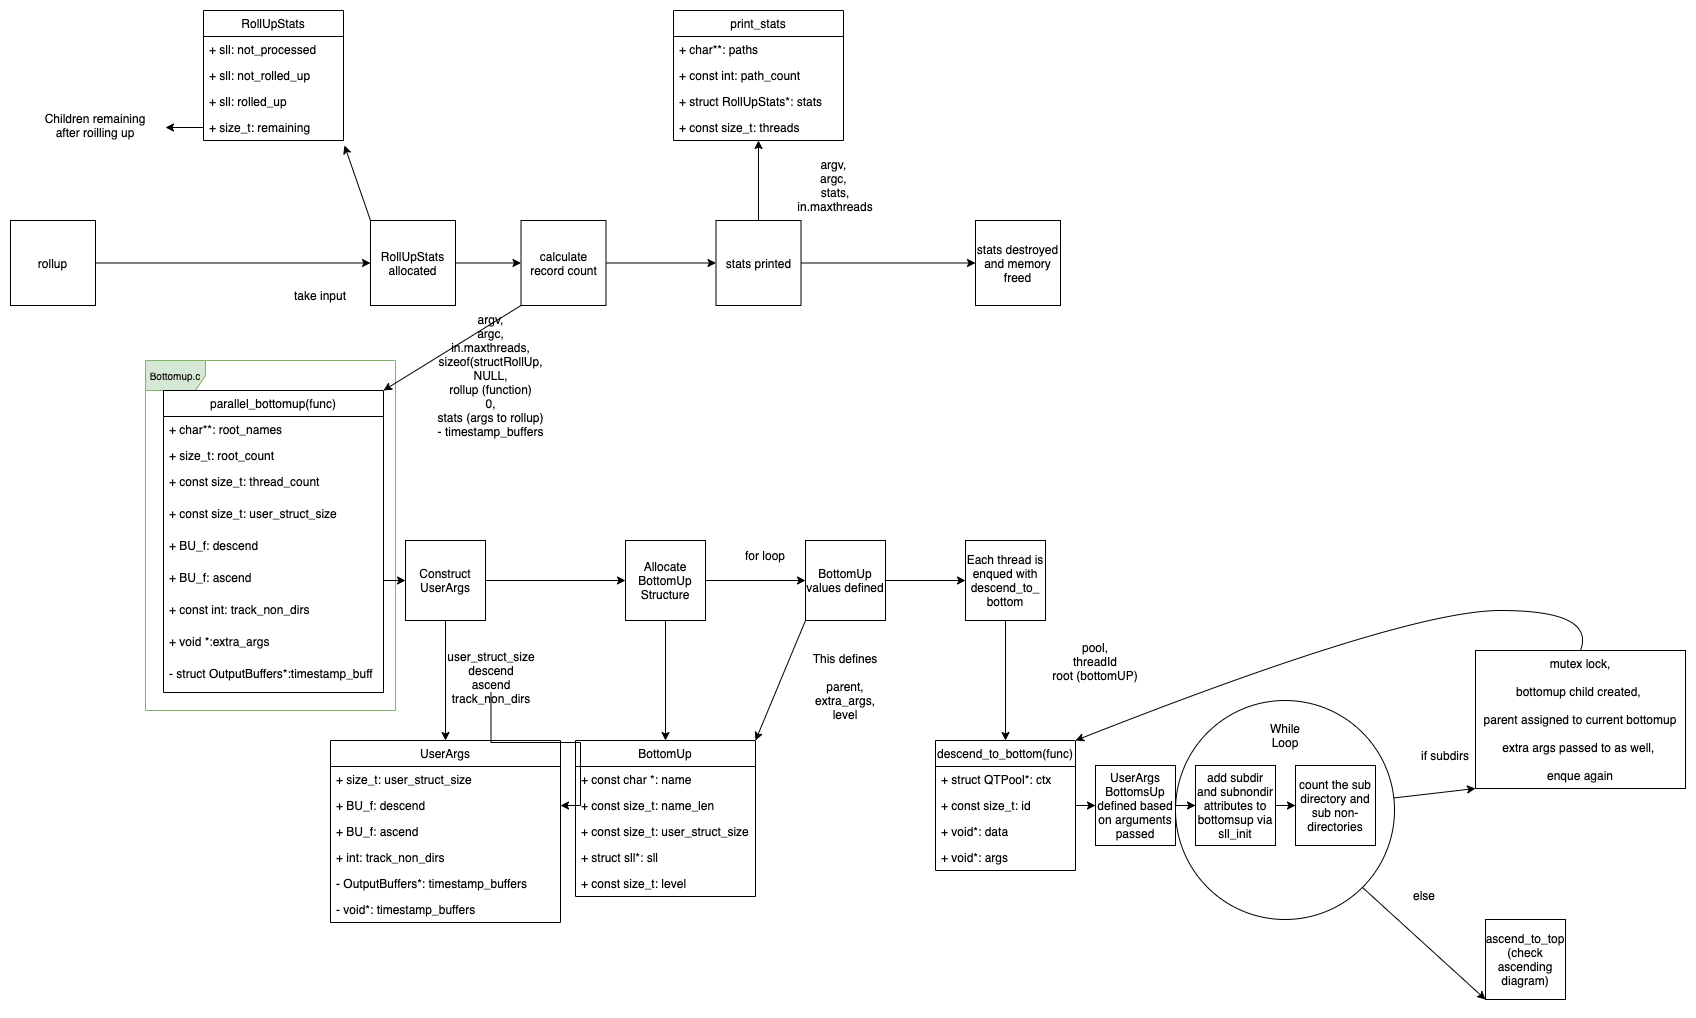
\includegraphics[width=\textwidth]{images/rollup.png}
  \caption{\rollup Workflow}
  \label{fig:rollupworkflow}
\end{sidewaysfigure}

\begin{figure} [!htb]
  \centering
  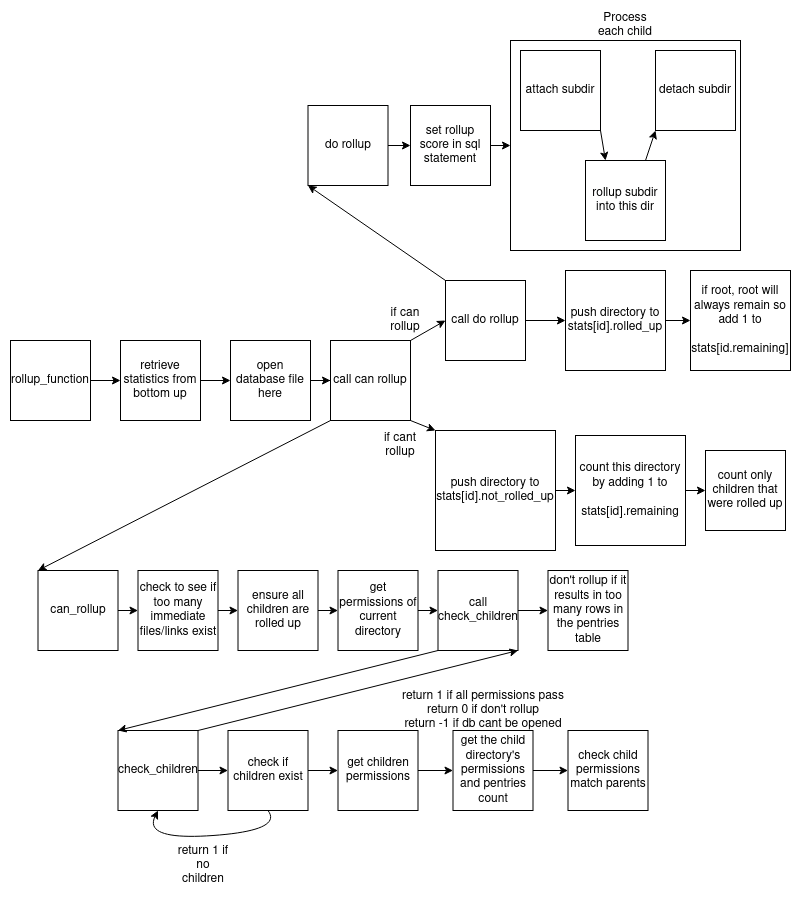
\includegraphics[width=\textwidth]{images/rollup_function.png}
  \caption{Rollup Function Diagram}
  \label{fig:rollupfunction}
\end{figure}

\subsection{Undoing a rollup}
To remove rollup data from an index, run the \unrollup executable:
\\\\
\indent \unrollup \texttt{[index root]}

% This file is part of GUFI, which is part of MarFS, which is released
% under the BSD license.
%
%
% Copyright (c) 2017, Los Alamos National Security (LANS), LLC
% All rights reserved.
%
% Redistribution and use in source and binary forms, with or without modification,
% are permitted provided that the following conditions are met:
%
% 1. Redistributions of source code must retain the above copyright notice, this
% list of conditions and the following disclaimer.
%
% 2. Redistributions in binary form must reproduce the above copyright notice,
% this list of conditions and the following disclaimer in the documentation and/or
% other materials provided with the distribution.
%
% 3. Neither the name of the copyright holder nor the names of its contributors
% may be used to endorse or promote products derived from this software without
% specific prior written permission.
%
% THIS SOFTWARE IS PROVIDED BY THE COPYRIGHT HOLDERS AND CONTRIBUTORS "AS IS" AND
% ANY EXPRESS OR IMPLIED WARRANTIES, INCLUDING, BUT NOT LIMITED TO, THE IMPLIED
% WARRANTIES OF MERCHANTABILITY AND FITNESS FOR A PARTICULAR PURPOSE ARE DISCLAIMED.
% IN NO EVENT SHALL THE COPYRIGHT HOLDER OR CONTRIBUTORS BE LIABLE FOR ANY DIRECT,
% INDIRECT, INCIDENTAL, SPECIAL, EXEMPLARY, OR CONSEQUENTIAL DAMAGES (INCLUDING,
% BUT NOT LIMITED TO, PROCUREMENT OF SUBSTITUTE GOODS OR SERVICES; LOSS OF USE,
% DATA, OR PROFITS; OR BUSINESS INTERRUPTION) HOWEVER CAUSED AND ON ANY THEORY OF
% LIABILITY, WHETHER IN CONTRACT, STRICT LIABILITY, OR TORT (INCLUDING NEGLIGENCE
% OR OTHERWISE) ARISING IN ANY WAY OUT OF THE USE OF THIS SOFTWARE, EVEN IF
% ADVISED OF THE POSSIBILITY OF SUCH DAMAGE.
%
%
% From Los Alamos National Security, LLC:
% LA-CC-15-039
%
% Copyright (c) 2017, Los Alamos National Security, LLC All rights reserved.
% Copyright 2017. Los Alamos National Security, LLC. This software was produced
% under U.S. Government contract DE-AC52-06NA25396 for Los Alamos National
% Laboratory (LANL), which is operated by Los Alamos National Security, LLC for
% the U.S. Department of Energy. The U.S. Government has rights to use,
% reproduce, and distribute this software.  NEITHER THE GOVERNMENT NOR LOS
% ALAMOS NATIONAL SECURITY, LLC MAKES ANY WARRANTY, EXPRESS OR IMPLIED, OR
% ASSUMES ANY LIABILITY FOR THE USE OF THIS SOFTWARE.  If software is
% modified to produce derivative works, such modified software should be
% clearly marked, so as not to confuse it with the version available from
% LANL.
%
% THIS SOFTWARE IS PROVIDED BY LOS ALAMOS NATIONAL SECURITY, LLC AND CONTRIBUTORS
% "AS IS" AND ANY EXPRESS OR IMPLIED WARRANTIES, INCLUDING, BUT NOT LIMITED TO,
% THE IMPLIED WARRANTIES OF MERCHANTABILITY AND FITNESS FOR A PARTICULAR PURPOSE
% ARE DISCLAIMED. IN NO EVENT SHALL LOS ALAMOS NATIONAL SECURITY, LLC OR
% CONTRIBUTORS BE LIABLE FOR ANY DIRECT, INDIRECT, INCIDENTAL, SPECIAL,
% EXEMPLARY, OR CONSEQUENTIAL DAMAGES (INCLUDING, BUT NOT LIMITED TO, PROCUREMENT
% OF SUBSTITUTE GOODS OR SERVICES; LOSS OF USE, DATA, OR PROFITS; OR BUSINESS
% INTERRUPTION) HOWEVER CAUSED AND ON ANY THEORY OF LIABILITY, WHETHER IN
% CONTRACT, STRICT LIABILITY, OR TORT (INCLUDING NEGLIGENCE OR OTHERWISE) ARISING
% IN ANY WAY OUT OF THE USE OF THIS SOFTWARE, EVEN IF ADVISED OF THE POSSIBILITY
% OF SUCH DAMAGE.



\section{Extended Attributes}
\label{sec:xattrs}
GUFI supports the indexing and querying of user data through extended
attributes (xattrs).

Reading standard filesystem permissions of files only requires read
(and execute) access to the directory. Extended attribute names are
visible this way. However, because xattr values are user defined data,
their permissions are checked at the file level, requiring changes to
how GUFI stores data. For more information on xattrs, see
\texttt{xattr(7)}, \listxattr, and \getxattr.

\subsection{Indexing}
Directories containing files from multiple users might have xattrs
that are not readable by all who can view the \lstat data of the
directory. As GUFI was originally designed to only use directory-level
permission checks, a number of modifications were made to process
xattrs without violating their permissions.

\subsubsection{Roll In Rules}
Xattrs that are readable by all who have access to the directory are
stored in the \xattrspwd table in the main database. These xattrs are
referred to as ``rolled in''.

The rules that determine whether or not an xattr pair can roll in are
as follows:

\begin{itemize}
\item File is 0+R
\item File is UG+R doesnt matter on other, with file and parent same
  usr and grp and parent has only UG+R with no other read
\item File is U+R doesnt matter on grp and other, with file and parent
  same usr and parent dir has only U+R, no grp and other read
\item Directory has write for every read:
    \texttt{drw*rw*rw*} or \texttt{drw*rw*\_\_\_} or
    \texttt{drw*\_\_\_\_\_\_} - if you can write the dir you can
    chmod the files to see the xattrs
\end{itemize}

Xattrs that cannot be read by all who can read the directory are
stored in external per-uid and per-gid databases set with
\texttt{uid:nobody} and \texttt{nobody:gid} owners respectively. This
makes it so that non-admin users cannot access the xattrs stored in
external databases that they do not have permissions to access.

\subsubsection{Schema}
\label{sec:xattr_schema}
The main database and all external databases contain the following
tables and views:

\begin{itemize}
\item The \xattrspwd table contains all extended attributes of the
  current directory that were placed into this database file.

\item The \xattrsrollup table contains all extended attributes that
  were placed into the children directories that were subsequently
  rolled up into the current directory.

\item The \xattrsavail view is the union of all extended attributes
  in \xattrspwd and \xattrsrollup in this database file.
\end{itemize}

Additionally, each main database file has the following tables and
views in order to keep track of which files were created by GUFI for
the purposes of storing xattrs:

\begin{itemize}
\item The \xattrfilespwd table contains a listing of external database
  filenames that contain xattrs that were not rolled in.
\item The \xattrfilesrollup table contains a listing of external
  database filenames that contain xattrs that were not
  rolled in, but were brought in by rolling up.
\item The \xattrfiles view combines the listings of database filenames
  found in \xattrfilespwd and \xattrfilesrollup.
\end{itemize}

\subsubsection{Usage}
Extended attributes are not pulled from the filesystem by default. In
order to pull them, pass \texttt{-x} to \gufidirindex or
\gufidirtrace.

Note that only xattr pairs in the user namespace (\texttt{user.*}) are
extracted.

\subsubsection{Rollup}
Additional steps were added to rollups in order to copy rolled up
xattrs upwards properly:

\begin{itemize}
\item The child's \xattrsavail view (without external database data)
  is copied into the parent's \xattrsrollup table.
\item The child's \xattrfiles view (without external databases data)
  is copied into the parent's \xattrfilesrollup table.
\item The child's external database files are copied into the
  parent. If the parent already has an external database file with the
  same uid or gid, the contents of the external database are copied
  into the parent's external database's \xattrsrollup table instead.
\end{itemize}

\subsection{Querying}
When querying for xattrs, pass \texttt{-x} to \gufiquery to build the
\xattrs view for querying. This view is a SQL union of rolled in
xattrs and any external databases that successfully
attaches. Attaching the database files checks the permissions of the
xattrs. \texttt{UNION} removes duplicate entries that showed up in
multiple external databases, leaving a unique set of xattrs accessible
by the caller.

The \xentries, \xpentries, \xsummary views are convenience views
generated so that users do not have to perform joins themselves. Like
the \xattrs view, these views are also dropped at the end of directory
processing.

Note that entries with multiple extended attributes will return
multiple times in this view.

% This file is part of GUFI, which is part of MarFS, which is released
% under the BSD license.
%
%
% Copyright (c) 2017, Los Alamos National Security (LANS), LLC
% All rights reserved.
%
% Redistribution and use in source and binary forms, with or without modification,
% are permitted provided that the following conditions are met:
%
% 1. Redistributions of source code must retain the above copyright notice, this
% list of conditions and the following disclaimer.
%
% 2. Redistributions in binary form must reproduce the above copyright notice,
% this list of conditions and the following disclaimer in the documentation and/or
% other materials provided with the distribution.
%
% 3. Neither the name of the copyright holder nor the names of its contributors
% may be used to endorse or promote products derived from this software without
% specific prior written permission.
%
% THIS SOFTWARE IS PROVIDED BY THE COPYRIGHT HOLDERS AND CONTRIBUTORS "AS IS" AND
% ANY EXPRESS OR IMPLIED WARRANTIES, INCLUDING, BUT NOT LIMITED TO, THE IMPLIED
% WARRANTIES OF MERCHANTABILITY AND FITNESS FOR A PARTICULAR PURPOSE ARE DISCLAIMED.
% IN NO EVENT SHALL THE COPYRIGHT HOLDER OR CONTRIBUTORS BE LIABLE FOR ANY DIRECT,
% INDIRECT, INCIDENTAL, SPECIAL, EXEMPLARY, OR CONSEQUENTIAL DAMAGES (INCLUDING,
% BUT NOT LIMITED TO, PROCUREMENT OF SUBSTITUTE GOODS OR SERVICES; LOSS OF USE,
% DATA, OR PROFITS; OR BUSINESS INTERRUPTION) HOWEVER CAUSED AND ON ANY THEORY OF
% LIABILITY, WHETHER IN CONTRACT, STRICT LIABILITY, OR TORT (INCLUDING NEGLIGENCE
% OR OTHERWISE) ARISING IN ANY WAY OUT OF THE USE OF THIS SOFTWARE, EVEN IF
% ADVISED OF THE POSSIBILITY OF SUCH DAMAGE.
%
%
% From Los Alamos National Security, LLC:
% LA-CC-15-039
%
% Copyright (c) 2017, Los Alamos National Security, LLC All rights reserved.
% Copyright 2017. Los Alamos National Security, LLC. This software was produced
% under U.S. Government contract DE-AC52-06NA25396 for Los Alamos National
% Laboratory (LANL), which is operated by Los Alamos National Security, LLC for
% the U.S. Department of Energy. The U.S. Government has rights to use,
% reproduce, and distribute this software.  NEITHER THE GOVERNMENT NOR LOS
% ALAMOS NATIONAL SECURITY, LLC MAKES ANY WARRANTY, EXPRESS OR IMPLIED, OR
% ASSUMES ANY LIABILITY FOR THE USE OF THIS SOFTWARE.  If software is
% modified to produce derivative works, such modified software should be
% clearly marked, so as not to confuse it with the version available from
% LANL.
%
% THIS SOFTWARE IS PROVIDED BY LOS ALAMOS NATIONAL SECURITY, LLC AND CONTRIBUTORS
% "AS IS" AND ANY EXPRESS OR IMPLIED WARRANTIES, INCLUDING, BUT NOT LIMITED TO,
% THE IMPLIED WARRANTIES OF MERCHANTABILITY AND FITNESS FOR A PARTICULAR PURPOSE
% ARE DISCLAIMED. IN NO EVENT SHALL LOS ALAMOS NATIONAL SECURITY, LLC OR
% CONTRIBUTORS BE LIABLE FOR ANY DIRECT, INDIRECT, INCIDENTAL, SPECIAL,
% EXEMPLARY, OR CONSEQUENTIAL DAMAGES (INCLUDING, BUT NOT LIMITED TO, PROCUREMENT
% OF SUBSTITUTE GOODS OR SERVICES; LOSS OF USE, DATA, OR PROFITS; OR BUSINESS
% INTERRUPTION) HOWEVER CAUSED AND ON ANY THEORY OF LIABILITY, WHETHER IN
% CONTRACT, STRICT LIABILITY, OR TORT (INCLUDING NEGLIGENCE OR OTHERWISE) ARISING
% IN ANY WAY OUT OF THE USE OF THIS SOFTWARE, EVEN IF ADVISED OF THE POSSIBILITY
% OF SUCH DAMAGE.



\section{Querying}
Once an index has been created, it should be queried using GUFI tools.

\section{gufi\_query}

\subsection{Outline}

gufi\_query is used in order to query information from the generated databases that include all of the information about the indexed root directory and its sub-directories while also taking into account permissions 
\subsection{Flags}

\begin{table} [h]
\centering
\begin{tabular}{l|p{6cm}}
Flag & Functionality \\\hline
-h & help\\
\hline
-H & show assigned input values (debugging)\\
\hline
-E \textless SQL ent\textgreater & SQL for entries table \\
\hline
-S \textless SQL sum\textgreater (will be read first) & SQL for summary table\\
\hline
-T \textless SQL tsum\textgreater & SQL for tree-summary table\\
\hline
-a & AND/OR (SQL query combination)\\
\hline
-n \textless threads\textgreater & number of threads\\
\hline
-j & print the information in terse form\\
\hline
-o \textless out\_fname\textgreater & output file (one-per thread, with thread-id suffix) implies -e 1\\
\hline
-d \textless delim\textgreater & one char delimiter \\
\hline
-O \textless out\_DB\textgreater & output DB, implies -e 1 \\
\hline
-I \textless SQL\_init\textgreater & SQL init \\
\hline
-F \textless SQL\_fin\textgreater & SQL cleanup \\
\hline
-y \textless min-level\textgreater & minimum level to descend to \\
\hline
-z \textless max-level\textgreater & maximum level to descend to\\
\hline
-J \textless SQL\_interm\textgreater & SQL for intermediate results (no default: recommend using "SELECT * FROM entries") \\
\hline
-K \textless create aggregate\textgreater & SQL to create the final aggregation table (if not specified, -I will be used)\\
\hline
-G \textless SQL\_aggregate\textgreater & SQL for aggregated results (no default: recommend using "SELECT * FROM entries")\\
\hline
-e \textless 0 or 1\textgreater & 0 for aggregate, 1 for print without aggregating (implied by -o and -O)\\
\hline
-m & Keep mtime and atime same on the database files \\
\hline
-B \textless buffer size\textgreater & size of each thread's output buffer in bytes \\
\hline
-w & open the database files in read-write mode instead of read only mode
\end{tabular}
\caption{\label{tab:widgets}Flags and Arguments}
\end{table}

\clearpage

\subsection{Example Calls}

gufi\_query -S "SELECT * FROM summary" ~/directory\_of\_root\_index
\\
gufi\_query -E "SELECT * FROM pentries" ~/directory\_of\_root\_index


\subsection{Visualizing the Workflow}


\begin{figure} [h]
\centering
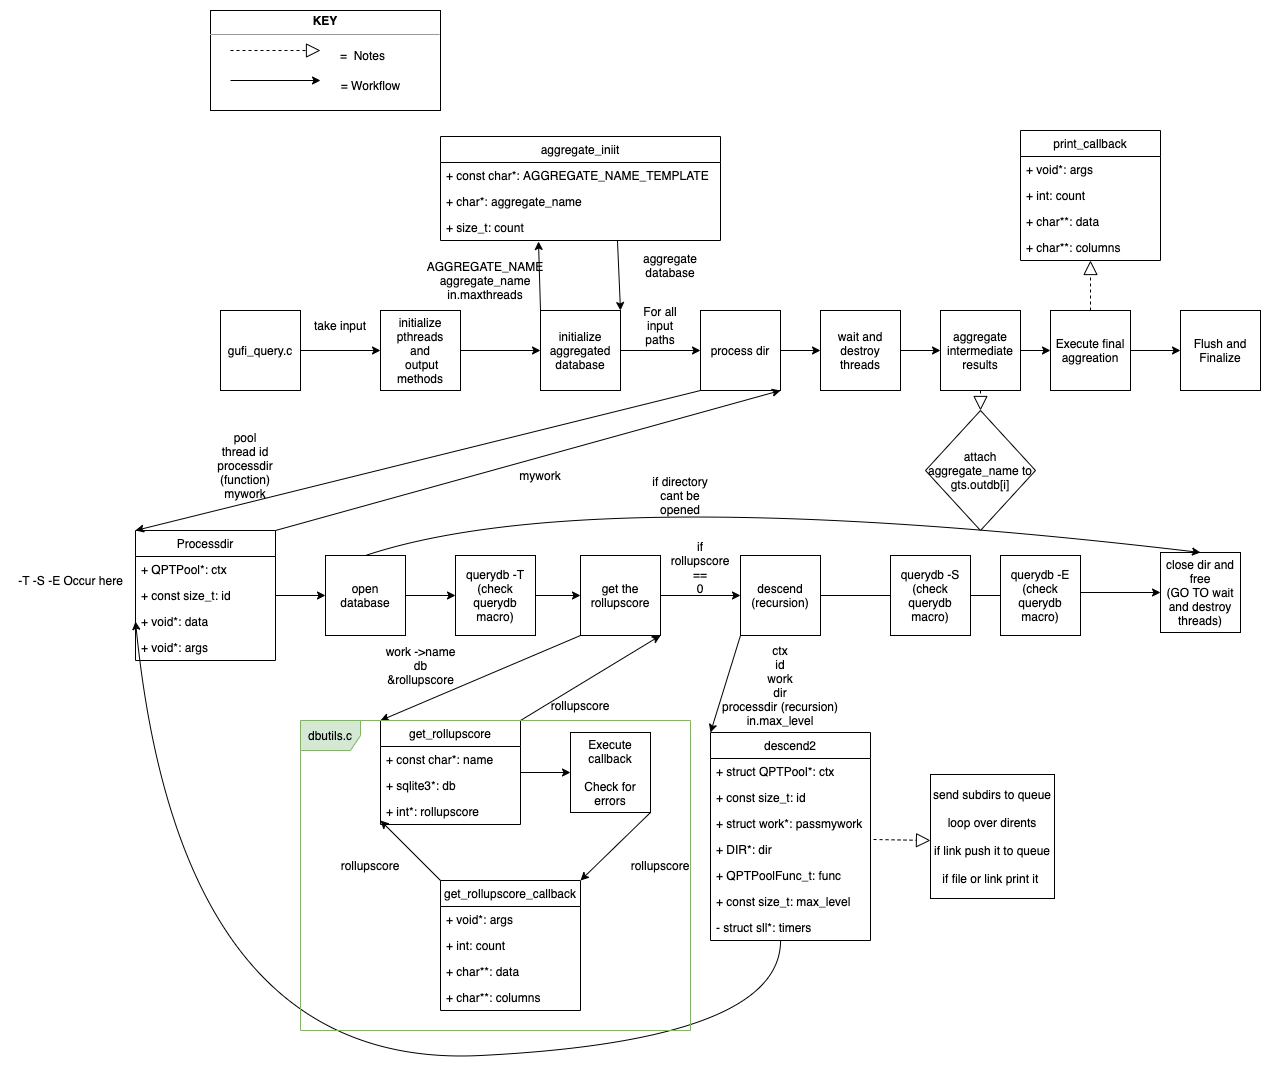
\includegraphics[width=1.0\textwidth]{images/gufi_query.png}
\caption{\label{fig:gufi_query}Workflow of gufi\_query}
\end{figure}


% This file is part of GUFI, which is part of MarFS, which is released
% under the BSD license.
%
%
% Copyright (c) 2017, Los Alamos National Security (LANS), LLC
% All rights reserved.
%
% Redistribution and use in source and binary forms, with or without modification,
% are permitted provided that the following conditions are met:
%
% 1. Redistributions of source code must retain the above copyright notice, this
% list of conditions and the following disclaimer.
%
% 2. Redistributions in binary form must reproduce the above copyright notice,
% this list of conditions and the following disclaimer in the documentation and/or
% other materials provided with the distribution.
%
% 3. Neither the name of the copyright holder nor the names of its contributors
% may be used to endorse or promote products derived from this software without
% specific prior written permission.
%
% THIS SOFTWARE IS PROVIDED BY THE COPYRIGHT HOLDERS AND CONTRIBUTORS "AS IS" AND
% ANY EXPRESS OR IMPLIED WARRANTIES, INCLUDING, BUT NOT LIMITED TO, THE IMPLIED
% WARRANTIES OF MERCHANTABILITY AND FITNESS FOR A PARTICULAR PURPOSE ARE DISCLAIMED.
% IN NO EVENT SHALL THE COPYRIGHT HOLDER OR CONTRIBUTORS BE LIABLE FOR ANY DIRECT,
% INDIRECT, INCIDENTAL, SPECIAL, EXEMPLARY, OR CONSEQUENTIAL DAMAGES (INCLUDING,
% BUT NOT LIMITED TO, PROCUREMENT OF SUBSTITUTE GOODS OR SERVICES; LOSS OF USE,
% DATA, OR PROFITS; OR BUSINESS INTERRUPTION) HOWEVER CAUSED AND ON ANY THEORY OF
% LIABILITY, WHETHER IN CONTRACT, STRICT LIABILITY, OR TORT (INCLUDING NEGLIGENCE
% OR OTHERWISE) ARISING IN ANY WAY OUT OF THE USE OF THIS SOFTWARE, EVEN IF
% ADVISED OF THE POSSIBILITY OF SUCH DAMAGE.
%
%
% From Los Alamos National Security, LLC:
% LA-CC-15-039
%
% Copyright (c) 2017, Los Alamos National Security, LLC All rights reserved.
% Copyright 2017. Los Alamos National Security, LLC. This software was produced
% under U.S. Government contract DE-AC52-06NA25396 for Los Alamos National
% Laboratory (LANL), which is operated by Los Alamos National Security, LLC for
% the U.S. Department of Energy. The U.S. Government has rights to use,
% reproduce, and distribute this software.  NEITHER THE GOVERNMENT NOR LOS
% ALAMOS NATIONAL SECURITY, LLC MAKES ANY WARRANTY, EXPRESS OR IMPLIED, OR
% ASSUMES ANY LIABILITY FOR THE USE OF THIS SOFTWARE.  If software is
% modified to produce derivative works, such modified software should be
% clearly marked, so as not to confuse it with the version available from
% LANL.
%
% THIS SOFTWARE IS PROVIDED BY LOS ALAMOS NATIONAL SECURITY, LLC AND CONTRIBUTORS
% "AS IS" AND ANY EXPRESS OR IMPLIED WARRANTIES, INCLUDING, BUT NOT LIMITED TO,
% THE IMPLIED WARRANTIES OF MERCHANTABILITY AND FITNESS FOR A PARTICULAR PURPOSE
% ARE DISCLAIMED. IN NO EVENT SHALL LOS ALAMOS NATIONAL SECURITY, LLC OR
% CONTRIBUTORS BE LIABLE FOR ANY DIRECT, INDIRECT, INCIDENTAL, SPECIAL,
% EXEMPLARY, OR CONSEQUENTIAL DAMAGES (INCLUDING, BUT NOT LIMITED TO, PROCUREMENT
% OF SUBSTITUTE GOODS OR SERVICES; LOSS OF USE, DATA, OR PROFITS; OR BUSINESS
% INTERRUPTION) HOWEVER CAUSED AND ON ANY THEORY OF LIABILITY, WHETHER IN
% CONTRACT, STRICT LIABILITY, OR TORT (INCLUDING NEGLIGENCE OR OTHERWISE) ARISING
% IN ANY WAY OUT OF THE USE OF THIS SOFTWARE, EVEN IF ADVISED OF THE POSSIBILITY
% OF SUCH DAMAGE.



\subsection{\querydbs}
\querydbs attaches all database files it is given into a single view
for querying. All tables in the provided database files should have
the same name and schema. For tables called \texttt{table}, the view
combining all tables will be named \texttt{vtable}.

Note that there is
a hard limit of 125 databases that can be queried by querydbs that is
set by SQLite3.


% This file is part of GUFI, which is part of MarFS, which is released
% under the BSD license.
%
%
% Copyright (c) 2017, Los Alamos National Security (LANS), LLC
% All rights reserved.
%
% Redistribution and use in source and binary forms, with or without modification,
% are permitted provided that the following conditions are met:
%
% 1. Redistributions of source code must retain the above copyright notice, this
% list of conditions and the following disclaimer.
%
% 2. Redistributions in binary form must reproduce the above copyright notice,
% this list of conditions and the following disclaimer in the documentation and/or
% other materials provided with the distribution.
%
% 3. Neither the name of the copyright holder nor the names of its contributors
% may be used to endorse or promote products derived from this software without
% specific prior written permission.
%
% THIS SOFTWARE IS PROVIDED BY THE COPYRIGHT HOLDERS AND CONTRIBUTORS "AS IS" AND
% ANY EXPRESS OR IMPLIED WARRANTIES, INCLUDING, BUT NOT LIMITED TO, THE IMPLIED
% WARRANTIES OF MERCHANTABILITY AND FITNESS FOR A PARTICULAR PURPOSE ARE DISCLAIMED.
% IN NO EVENT SHALL THE COPYRIGHT HOLDER OR CONTRIBUTORS BE LIABLE FOR ANY DIRECT,
% INDIRECT, INCIDENTAL, SPECIAL, EXEMPLARY, OR CONSEQUENTIAL DAMAGES (INCLUDING,
% BUT NOT LIMITED TO, PROCUREMENT OF SUBSTITUTE GOODS OR SERVICES; LOSS OF USE,
% DATA, OR PROFITS; OR BUSINESS INTERRUPTION) HOWEVER CAUSED AND ON ANY THEORY OF
% LIABILITY, WHETHER IN CONTRACT, STRICT LIABILITY, OR TORT (INCLUDING NEGLIGENCE
% OR OTHERWISE) ARISING IN ANY WAY OUT OF THE USE OF THIS SOFTWARE, EVEN IF
% ADVISED OF THE POSSIBILITY OF SUCH DAMAGE.
%
%
% From Los Alamos National Security, LLC:
% LA-CC-15-039
%
% Copyright (c) 2017, Los Alamos National Security, LLC All rights reserved.
% Copyright 2017. Los Alamos National Security, LLC. This software was produced
% under U.S. Government contract DE-AC52-06NA25396 for Los Alamos National
% Laboratory (LANL), which is operated by Los Alamos National Security, LLC for
% the U.S. Department of Energy. The U.S. Government has rights to use,
% reproduce, and distribute this software.  NEITHER THE GOVERNMENT NOR LOS
% ALAMOS NATIONAL SECURITY, LLC MAKES ANY WARRANTY, EXPRESS OR IMPLIED, OR
% ASSUMES ANY LIABILITY FOR THE USE OF THIS SOFTWARE.  If software is
% modified to produce derivative works, such modified software should be
% clearly marked, so as not to confuse it with the version available from
% LANL.
%
% THIS SOFTWARE IS PROVIDED BY LOS ALAMOS NATIONAL SECURITY, LLC AND CONTRIBUTORS
% "AS IS" AND ANY EXPRESS OR IMPLIED WARRANTIES, INCLUDING, BUT NOT LIMITED TO,
% THE IMPLIED WARRANTIES OF MERCHANTABILITY AND FITNESS FOR A PARTICULAR PURPOSE
% ARE DISCLAIMED. IN NO EVENT SHALL LOS ALAMOS NATIONAL SECURITY, LLC OR
% CONTRIBUTORS BE LIABLE FOR ANY DIRECT, INDIRECT, INCIDENTAL, SPECIAL,
% EXEMPLARY, OR CONSEQUENTIAL DAMAGES (INCLUDING, BUT NOT LIMITED TO, PROCUREMENT
% OF SUBSTITUTE GOODS OR SERVICES; LOSS OF USE, DATA, OR PROFITS; OR BUSINESS
% INTERRUPTION) HOWEVER CAUSED AND ON ANY THEORY OF LIABILITY, WHETHER IN
% CONTRACT, STRICT LIABILITY, OR TORT (INCLUDING NEGLIGENCE OR OTHERWISE) ARISING
% IN ANY WAY OUT OF THE USE OF THIS SOFTWARE, EVEN IF ADVISED OF THE POSSIBILITY
% OF SUCH DAMAGE.



\section{Deployment}
\label{sec:deploy}
GUFI functionality as described so far has been local. However, users
are not expected to log into the machine with the indices with an
interactive shell. Instead, they are expected to call wrapper scripts
to forward commands to the server (installed with the client RPM).

\subsection{RPMs}
When client building is enabled and the rpms built (\texttt{make
  package}), two rpms will be created. The server rpm will contain
GUFI as described so far. The client rpm will contain executables that
should be installed on the client node. The user executables on the
client side simply forward commands to the server. A jailed shell
should be set up on the server to prevent arbitrary command execution
- see Section~\ref{sec:gufi_jail} for details.

\subsection{SSH}
Normal ssh, using passwords or user keys (\texttt{\textasciitilde
  /.ssh/id\_rsa}), should be disabled on the server. Instead, ssh
should be done using host based authentication
(\texttt{/etc/ssh/ssh\_host\_rsa\_key}).

\subsection{Runtime Configuration}
\gufiquery provides the core GUFI functionality. However it is not
expected to be used by users, as the syntax of \gufiquery is somewhat
unwieldy, and users are not expected to understand how GUFI
works. Wrappers were created in order to provide users (and
administrators) with predetermined queries that are used often and
extract useful information (see the user guide for more details). The
server has the actual implementation of the wrappers while the clients
have command forwarders.

These wrappers require configuration files located at
\guficonfigfile (with read permissions for all GUFI users)
to function. These configuration files are simple text files
containing lines of \texttt{<key>=<value>}. Duplicate configuration
keys are overwritten by the bottom-most line. Empty lines and lines
starting with \# are ignored. The server and client require different
configuration values. Example configuration files can be found in the
\texttt{config} directory of the GUFI source, as well as in the build
directory. The corresponding examples will also be installed with
GUFI.

If a server and client exist on the same node, the server and client
configuration file may be combined into one file.

\subsubsection{Server}
\begin{tabular}{| l | l | l |}
  \hline
  Key & Value Type & Purpose \\
  \hline
  Threads & Positive Integer & Number of threads to use \\
  & & when running \gufiquery. \\
  \hline
  Executable & File Path & The absolute path of \gufiquery. \\
  \hline
  IndexRoot & Directory Path & The absolute path of the GUFI index \\
  & & (or parent of multiple indices). \\
  \hline
  OutputBuffer & Non-negative Integer & The size of each per-thread
  buffer \\
  & & used to buffer writes to stdout. \\
  & & Setting this too low will affect \\
  & & performance. Setting this too high \\
  & & will use too much resources. \\
  \hline
\end{tabular}

\subsubsection{Client}
\begin{tabular}{| l | l | l |}
  \hline
  Key Value & Type & Purpose \\
  \hline
  Server & URI & The URI of the server (IP address, URL, etc.) \\
  \hline
  Port & Non-negative integer & Port number \\
  \hline
  Paramiko & Directory Path & The absolute path to the paramiko \\
  & & directory on the client side \\
  \hline
\end{tabular}

\subsection{\gufijail}
\label{sec:gufi_jail}
\gufijail is a simple script that limits the commands users logging in
with ssh are able to run to only a subset of GUFI
commands. \texttt{/etc/ssh/sshd\_config} should be modified with the
following lines:

\begin{verbatim}
    Match Group gufi
        ForceCommand /path/to/gufi_jail
\end{verbatim}


\end{document}
